\documentclass[a4paper,cleardoubleempty,BCOR1cm, 11pt]{report}
% use to waste space:
% \documentclass[12pt,a4paper]{article}

% if you have this style and like it.
%\documentclass{acmsiggraph}
%\documentclass[review]{acmsiggraph}      % review
%\documentclass[widereview]{acmsiggraph}  % wide-spaced review
%\documentclass[preprint]{acmsiggraph}    % preprint

% define a \comment{this is a comment which can have linebreaks in it}
\newcommand{\comment}[1]{}
% \newcommand{\todo}[1]{\marginpar{\bf{#1}}}
\newcommand{\todo}[1]{{\color{red}\bf{TODO: #1}}}
\usepackage{booktabs}
\usepackage{mathptmx}
\usepackage[pdftex]{graphicx}
\usepackage[pdftex]{color}
\definecolor{rot}{RGB}{165,30,55} %rote Farbe
\definecolor{lila}{RGB}{90,0,91} %rote Farbe
\definecolor{schwarz}{RGB}{0,0,0}
\graphicspath{{./images/}}
\usepackage{parskip}
\usepackage{amsmath}
\usepackage{dsfont}
\usepackage{pxfonts}
\usepackage{natbib}
\usepackage{setspace}

\usepackage[paper=a4paper,left=25mm,right=35mm,top=25mm,bottom=20mm, includehead, includefoot, twoside]{geometry}
\usepackage[T1]{fontenc}
\usepackage{textcomp}

% comment these two lines out if you don't want minion/myriad fonts.
% \usepackage[minionint,mathlf]{MinionPro}
% \renewcommand{\sfdefault}{Myriad-LF}
%\usepackage{Myriad}

% no page number on float pages, fixes problems with overlarge diagrams.
\usepackage{fancyhdr}
\pagestyle{fancy}
%\lhead{}
%\chead{}
%\rhead{}
%\lfoot{}
\fancyhf{}
\fancyhead[EL]{\nouppercase{\leftmark}}
\fancyhead[OR]{\nouppercase{\rightmark}}
\cfoot{}
%\fancyfoot[EL]{\iffloatpage{}{\thepage}}
%\fancyfoot[OR]{\iffloatpage{}{\thepage}}
\fancyfoot[EL]{\thepage}
\fancyfoot[OR]{\thepage}
\renewcommand{\headrulewidth}{0pt}
\renewcommand{\footrulewidth}{0pt}

%\usepackage{natbib}		% textual referencing
%\usepackage[numbers,super]{natbib}	% nice superscripts
%\bibliographystyle{chicago}	% shitty
%\bibliographystyle{alpha}	% abbr names and year in \cite
%\bibliographystyle{agsm}	% australian, need natbib
%\bibliographystyle{kluwer}	% need natbib
\bibliographystyle{apalike}	% lengthly
%\bibliographystyle{abbrv}	% minimal?

% use for german line breaking:
%\usepackage[ngerman]{babel}
\usepackage[T1]{fontenc}
\usepackage[utf8x]{inputenc}

% avoid us-style text color destruction:
\frenchspacing
\usepackage{microtype}

% have a nice framebox with border directly around the image:
\fboxsep 0pt
\newcommand{\fimg}[2]{\fbox{\includegraphics[width=#1]{#2}}}

\usepackage{theorem}
\theorembodyfont{\upshape}
\newtheorem{definition}{Definition}

\usepackage{listings}
\lstset{numbers=left, numberstyle=\tiny, basicstyle=\tiny, language=Python}
%\usepackage[boxruled]{algorithm2e}
\usepackage{algorithm,algorithmic}% http://ctan.org/pkg/algorithms
%\usepackage{hyperref}
\usepackage{url}
\usepackage{subfig}

\def\code#1{{\tt{#1}}}



\begin{document}
\vspace*{10ex}
Bachelorarbeit

{\huge\bf\textsf{Uncertainty in\\
		Recurrent Decision Tree Classifiers}}

\vspace*{30ex}

Eberhard Karls Universität Tübingen\\
Mathematisch-Naturwissenschaftliche Fakultät\\
Wilhelm-Schickard-Institut für Informatik\\
Explainable Machine Learning\\
Stefan Wezel,~ \verb+stefan.wezel@student.uni-tuebingen.de+,~ 2020

\vspace*{5ex}

\begin{tabular}{@{}l@{\hspace{2em}}l}
	Bearbeitungszeitraum:& von-bis \vspace*{5ex} \\
	Betreuer*in/Gutachter*in:& Prof. Dr. Zeynep Akata, Universität Tübingen\\
	Betreuer*in:& Stephan Alaniz, Max Planck Institut für Informatik
\end{tabular}

\thispagestyle{empty}
%\newpage
	

\setstretch{1.25}
%\begin{tabular}{lr}
%
\includegraphics[width=0.5\linewidth]{logo_sw} % logo bw
 
\includegraphics[width=0.5\linewidth]{UT_WBMW_Rot_4C} % logo red
 & \hspace{0.2\linewidth}
 \parbox{0.5\linewidth}{
   \large\bf\textsf{\color{schwarz}{Mathematisch-\\Naturwissenschaftliche\\Fakultät\\\\}}
   \hspace{-.144cm}\normalsize\textsf{\color{lila}{Explainable Machine Learning}}
   \vspace{0.6cm}
 }
\end{tabular}

\vspace*{10ex}
Bachelorarbeit

{\huge\bf\textsf{Uncertainty in Recurrent Decision Tree Classifiers}}

\vspace*{30ex}

Eberhard Karls Universität Tübingen\\
Mathematisch-Naturwissenschaftliche Fakultät\\
Wilhelm-Schickard-Institut für Informatik\\
Explainable Machine Learning\\
Stefan Wezel,~ \verb+stefan.wezel@student.uni-tuebingen.de+,~ 2020

\vspace*{5ex}

\begin{tabular}{@{}l@{\hspace{2em}}l}
  Bearbeitungszeitraum:& von-bis \vspace*{5ex} \\
  Betreuer/Gutachter:& Prof. Dr. Zeynep Akata, Universität Tübingen\\
  Betreuer:& Stephan Alaniz, Max Planck Institut für Informatik
\end{tabular}

\thispagestyle{empty}
\newpage

\chapter*{Selbstst\"andigkeitserkl\"arung}
Hiermit versichere ich, dass ich die vorliegende Bachelorarbeit selbst\"andig und
nur mit den angegebenen Hilfsmitteln angefertigt habe und dass alle Stellen,
die dem Wortlaut oder dem Sinne nach anderen Werken entnommen sind,
durch Angaben von Quellen als Entlehnung kenntlich gemacht worden sind.
Diese Bachelorarbeit wurde in gleicher oder \"ahnlicher Form in keinem anderen
Studiengang als Pr\"ufungsleistung vorgelegt.

\vspace*{8ex}
\hrule
\vspace*{2ex}
Stefan Wezel (Matrikelnummer 4080589), \today


\chapter*{Abstract}
Recurrent Decision Tree Classifiers (RDTC) have proven to be capable of providing explanations for their classifications while yielding state of the art results in prediction accuracy on several image classification tasks. However, they may utilize features that they are highly uncertain about. We hypothesize that when using uncertainty information, the RDTC can provide more faithful explanations and become more applicable in real-life scenarios.
Based on RDTC, we propose a model that utilizes uncertainty information. We either enhance the vocabulary of RDTC with an uncertainty token, allowing for a ternary decision tree, or, we restrict the RDTC from using uncertain attributes. 
We investigate how this uncertainty information can be used in generating interpretable model outputs and how it affects the model's performance on several benchmark tasks. We show that our model reliably yields high uncertainty for examples from unseen classes. Moreover its performance on benchmark image datasets is comparable to other State-of-the-art methods.





\tableofcontents

%% braucht kein Mensch ...
%\listoffigures
%\listoftables


\chapter{Introduction}
% Motivation for explainabiltiy and uncertainty
The recent surge in the popularity of machine learning methods has made the field's ambivalent nature obvious. Public opinion is split between hype and mistrust. 
Systems using machine learning have failed at seemingly simple tasks \cite{kelion2018ces}, displayed racist and sexist behavior \cite{guynn2015google, schlesinger2018let, zou2018ai}, and even caused fatalities \cite{yadron2016tesla}.
Such cases, where artificial intelligence has made severe mistakes are amusing at best and outright dangerous at worst. Most importantly, they have made it clear that, despite being deployed more frequently than ever before, machine learning has yet to prove itself \cite{schlesinger2018let, dikmen2016autonomous, zou2018ai}. 
These cases show that blind trust in black box models can lead to dangerous outcomes and that methods allowing introspection and behaving faithfully are more important than ever.\\
Addressing such issues, \citet{alaniz2019explainable} propose a model that can reliable justify its classification by stating utilized features in a decision tree. Here, we build on this method. We extend the model so that it is aware of and able to express its uncertainties. We hypothesize that such a model may be perceived by a user as more trustful than a model that does not.\\
% more motivation on uncertainty
Uncertainty information can help improve the interaction between artificial intelligence and users.
We, as humans have developed an intuition on how to make decisions under uncertainty \cite{bland2012different} and are able to operate in a domain of limited and noisy data. Moreover, uncertainty is an important measure in science that allows us to express how well something is known or can be known. Scientists from fields like medicine, physics, or meteorology rely on uncertainty information for making and communicating decisions or predictions. Outside the scientific world, uncertainty information is important in finance or law among others \cite{liu2013toward, d1983legal}.\\
Uncertainty information is valuable, especially in real-world scenarios, where we might encounter only limited or noisy data to learn from. Or, where decisions with high consequences have to be made. 
As machine learning becomes more prevalent in our everyday lives, in science, finance, or law, the need for methods, utilizing uncertainty becomes more evident.\\
% overconfidence of softmax and uncertainty
Unfortunately, the output of most neural network architectures does not contain uncertainty information. For example, in classification, typical architectures use a softmax layer, to turn model outputs into a probability density function over classes \cite{nwankpa2018activation}. Since it is a probability distribution, the softmax output is often misinterpreted as a measure of how certain a model is regarding each class \cite{sensoy2018evidential}. However, this distribution only arises from each value relative to every other value and is a point estimate, turned into a distribution. The point estimate cannot carry any uncertainty information and the softmax certainly does not add such information. This allows a softmax class probability to be overconfident for a highly uncertain class \cite{gal2016dropout}.\\
% Key contributions
Our key contributions are to propose a model, that allows to (1) study the effect of uncertainty for attribute-based recurrent decision tree classifier and actively uses and expresses uncertainty information. We (2) test the proposed model's performance on popular datasets and compare it to different state-of-the-art methods. We investigate uncertainties in the model and data and evaluate its effect on performance. \\
% Example applications
Such a model may be applied in settings where a high confidence classification for out-of-distribution (OOD) examples may have severe consequences, for example in medical settings, in law, or in autonomous driving. There, in cases of high uncertainty, a human could be notified and consulted, preventing the model from making a (potentially wrong) high-risk decision. The model would still provide a decision tree as an explanation, which could be utilized by a human user to make a final decision.




\chapter{Related Work}
Building on, often centuries-old, mathematical foundations and on more recent psychological and neurobiological insights, machine learning has evolved throughout the last decades and a vast corpus of literature has emerged from this development. Here we will briefly go over some historic aspects, introduce important concepts, and give an overview of the current state of explainable methods and uncertainty in machine learning. 


\section{Neural Networks}
Artificial neural networks (ANNs) have become an integral part in the lives of many. Inspired by the cognitive processes of the mammalian brain, several architectures, and learning algorithms have been proposed.

\subsection{Historical Context}
The idea of artificial intelligence (AI) is dating back to antiquity and was debated in various domains ranging from chemistry \cite{o1994alchemical} to philosophy and mathematics \cite{leibnizdissertatio}. A watershed moment in its development is marked by \citet{mcculloch1943logical}, who modeled a neuron in an approach that unified findings from neurophysiology and mathematics. Later, \citet{hebb19680} brought forward a theory of how the strengthening and weakening of connections between neurons encodes gained knowledge.  This idea was also applied in the perceptron \cite{rosenblatt1960perceptron} which could learn to distinguish linearly separable classes. 
\citet{marvin1969perceptrons} created a more powerful architecture through introducing a middle layer to the perceptron and thus invented the multilayer perceptron (MLP). They found that if this hidden layer had a non-linear activation function it could learn to classify not linearly separable data. This idea of many simple but connected units remains a key principle in ANNs.
However, simulating the behavior of neural networks requires many computations, and the sequential nature of hardware available at the time prohibited connectionist ideas to be applied in practice.\\
Over the decades, ANNs have risen and fallen in popularity among AI researchers. Different architectures and learning algorithms have been proposed but many failed to establish. Important milestones were \citet{rumelhart1986learning}, who extended learning rules to MLP's in the backpropagation algorithm, the Long short-term memory by \citet{hochreiter1997long}, and the convolutional neural net (CNN), proposed by \citet{lecun1995convolutional} which allowed to classify handwritten digits.\\
However, these methods still failed to establish themselves beyond the realm of research. The development of graphics processing units (GPUs) and the availability of large-scale datasets have caused this to change in the 2010s, when for some tasks ANNs have exceeded human performance \cite{ILSVRC15}.


\subsection{Multilayer Perceptron}\label{sec:MLP}
The MLP is a rather simple architecture. It consists of an input layer, an arbitrary number of hidden layers, and an output layer. Each neuron is typically connected to each neuron in the next layer through weighted connections. Thus, each neuron gets the weighted output from the last layer's neurons as input. Non-linear activation functions allow the network to learn not linearly separable problems. Their straightforward structure and effectiveness make MLP's a widely used tool \cite{beale1990neural}. In the RDTC model, MLP's are used to learn mappings from the complex output of other models to a simpler structure, that is, i.e. interpretable by a human.


\begin{figure}
	\centering
	\begin{minipage}[t]{0.45\textwidth}
		\centering
		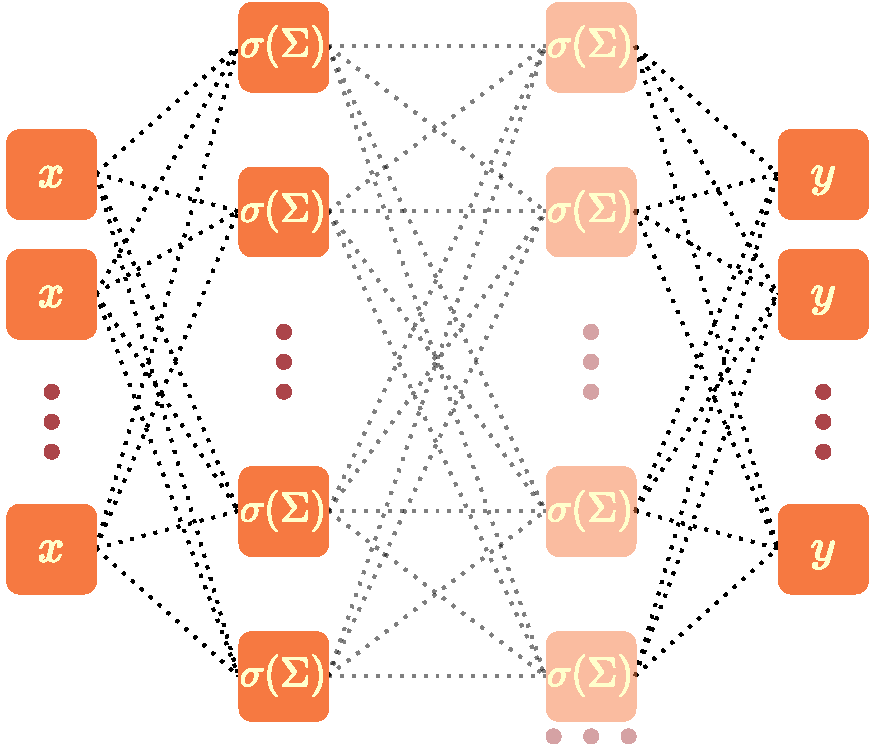
\includegraphics[width=0.8\textwidth,height=0.21\textheight]{images/mlp.pdf} 
		\caption{An MLP consists of an input layer, an arbitrary number of hidden layers, and an output layer. Hidden layers typically have non-linear activation functions.}
	\end{minipage}\hfill
	\begin{minipage}[t]{0.45\textwidth}
		\centering
		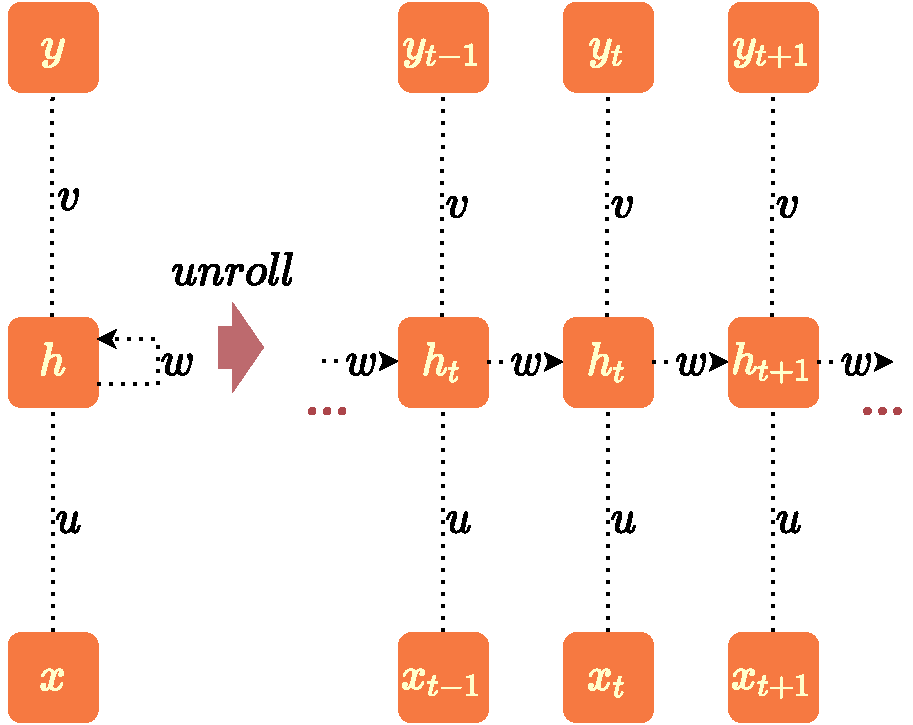
\includegraphics[width=0.9\textwidth,height=0.20\textheight]{images/rnn.pdf}
		\caption{The recurrent neural network takes in an input for every time step. Additionally it takes in its own hidden state from the last time step and computes an output for each time step.}
		\label{fig:rnn}
	\end{minipage}
\end{figure}




\subsection{Recurrent Neural Networks}
Many types of data do not provide samples of fixed size. This is the case for most language or time-series data among others. An MLP, however, is incapable of processing such samples due to its fixed amount of input neurons. RNN's process an input element by element in so called time steps and use values from previous time steps to compute outputs. This enables them to take in inputs of arbitrary length. Many concepts of RNN's exist \cite{Grossberg:2013}. Here we will have a closer look at the very simple example, depicted in Figure \ref{fig:rnn}.
The  RNN takes in an input $x_t$ which is transformed by weight matrix $u$ and added to the hidden state of the last time step times weight matrix $w$. This forms the hidden state of the current time step. To obtain an output at a given time step, the hidden state is multiplied with a weight matrix $v$. The update rules can be stated as:
\begin{align*}
	h_t &= f_{act}(u \circ x_t + w \circ h_{t-1})\\
	y_t &=f_{act}(v \circ h_t)
\end{align*}
An RNN can be trained by the Backpropagation through time algorithm (BPTT) \cite{werbos1990backpropagation}. \citet{werbos1990backpropagation} propose to unfold an RNN for each time step or element of the input. This unfolding makes it equivalent to a feed-forward ANN (such as the MLP introduced in Subsection \ref{sec:MLP}) and weights can be adjusted according to the gradients.\\
As basic RNN structures suffer from vanishing and exploding gradient problems \cite{bengio1994learning}, several improvements have been proposed such as the Long short-term memory (LSTM) \cite{hochreiter1997long} and the Gated recurrent unit (GRU) \cite{cho2014learning}.
The RDTC model relies on an LSTM to classify the decision tree which updates its depth after each question is asked and answered. This dynamically generated tree could not be classified by an MLP.


\subsection{Convolutional Neural Networks}
CNN's have proven to be a useful tool for various image-related tasks. They are a type of feed-forward network with the underlying concept of learning filters that correspond to features in the data. Typically this is done over multiple layers to learn to recognize low-level concepts such as edges in layers close to the input layer and high-level concepts in layers further away from the input. In practice, after convolutions and non-linearities are applied, the results are usually subsampled, using a pooling operation to reduce the number of necessary parameters. The RDTC model uses a CNN to learn to extract features from images.

\begin{figure}
	\centering
		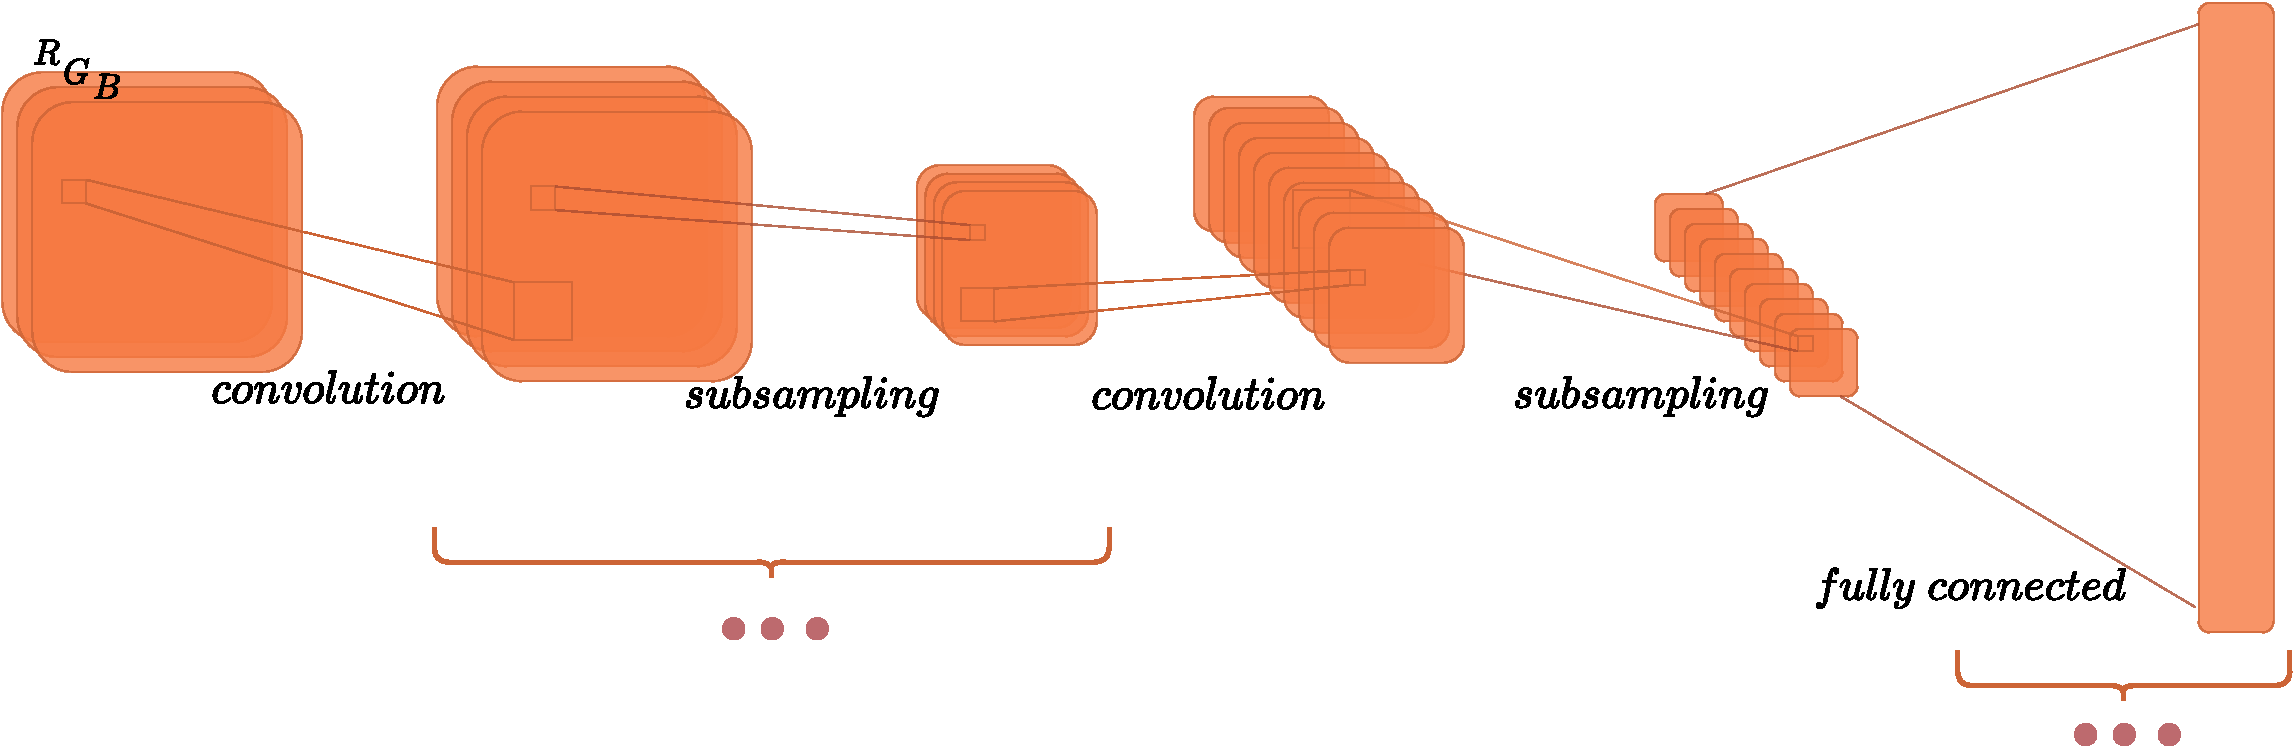
\includegraphics[width=0.9\textwidth]{images/convnet.pdf} 
		\caption{A CNN with two convolutional and subsampling layers. A fully connected layer transforms the learned features into a human interpretable output. The displayed structures can be repeated an arbitrary number of times. Modern convolutional architectures may have a large number of layers \cite{he2016deep,szegedy2015going,xie2017aggregated}.}
		\label{fig:convnet}
\end{figure}


\section{Explainable Machine Learning}
While interpretable models exist in machine learning, they are often outperformed by modern ANNs with a large number of parameters, on a variety of tasks \cite{gunning2019xai, guo2020explainable, sarkar2016accuracy, puiutta2020explainable}. Understanding the processes inside a model with a large number of parameters is not trivial. Thus, various approaches have been developed to understand a model's decision process for given data. Such methods, that are interpretable or can explain their decisions are inevitable for safety-critical applications. They allow a human user to understand how a model came to a certain output and allow for a faithful human-AI interaction to emerge.


\subsection{Decision Trees}
Decisions trees provide an inherently interpretable model. Given data with features $a_1, ..., a_n$ a decision tree iteratively splits data according to conditions for each attribute. Splits occur for each attribute $a_i$ where samples from data are either above or below a given threshold for their values of $a_i$. Optimal splits can be found by learning algorithms or by expert knowledge. Nodes represent the resulting splits and edges represent the corresponding answer.
Decision trees are a frequently used tool in data mining \cite{wu2008top}. Popular algorithms to generate decision trees from data include Iterative Dichotomiser 3 and C4.5, both suggested by Quinlan \cite{quinlan1986induction,quinlan2014c4}.
Another popular algorithm is Classification and Regression Trees, introduced by \citet{breiman1984classification}. The key concept behind these algorithms is to create splits that maximize information gain for each available attribute.\\
To reduce the size and increase the interpretability of generated trees, pruning can be applied \cite{mingers1989empirical}. Pruning can also reduce the risk of overfitting \cite{kearns1998fast}.\\
The RDTC builds a decision tree by asking questions about the presence of attributes in a given image. %Questions by the RDT can be viewed as nodes and the AbL's answers as edges.

\begin{figure}
	\centering
	\begin{minipage}[t]{0.45\textwidth}
		\centering
		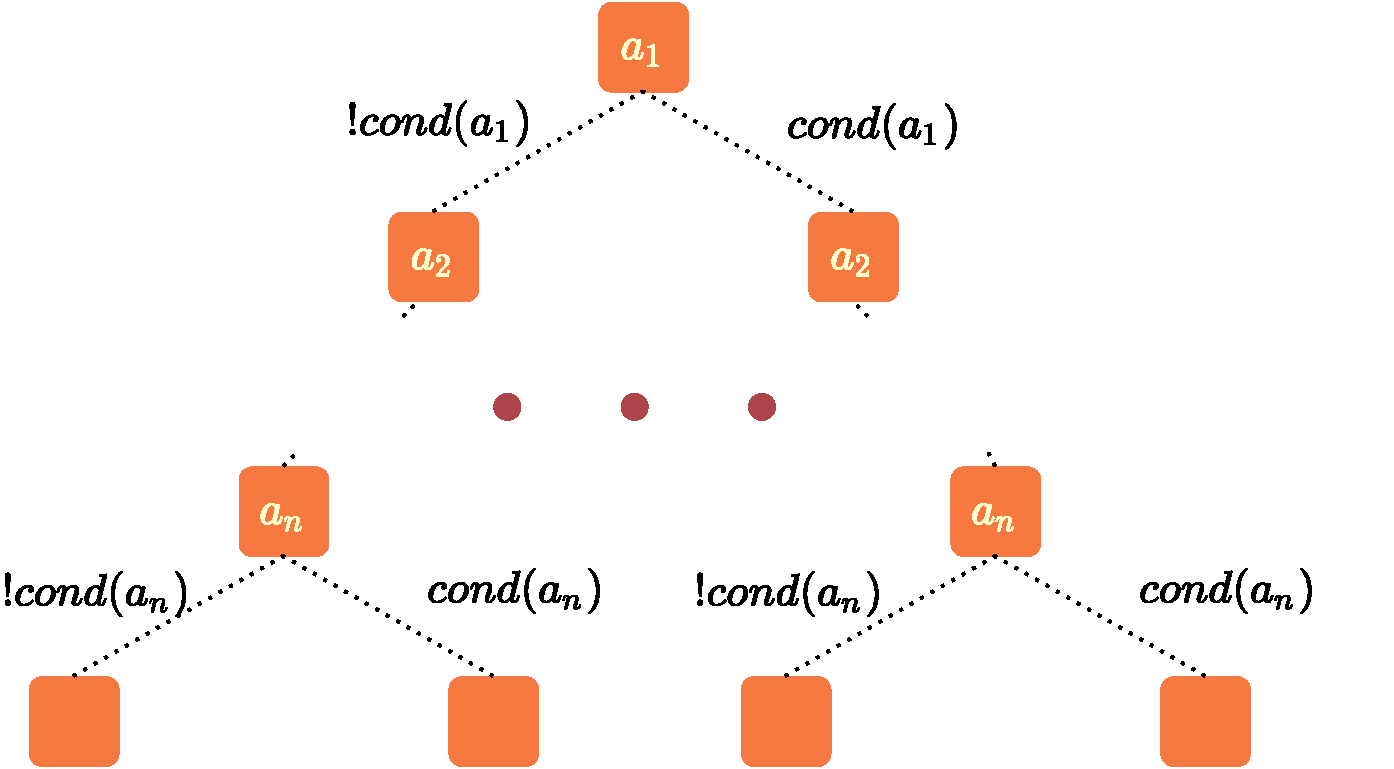
\includegraphics[width=0.9\textwidth,height=0.16\textheight]{images/decisiontree.pdf} 
		\caption{A decision tree splits data according to values of attributes.}
		\label{fig:decision_tree}
	\end{minipage}\hfill
	\begin{minipage}[t]{0.45\textwidth}
		\centering
		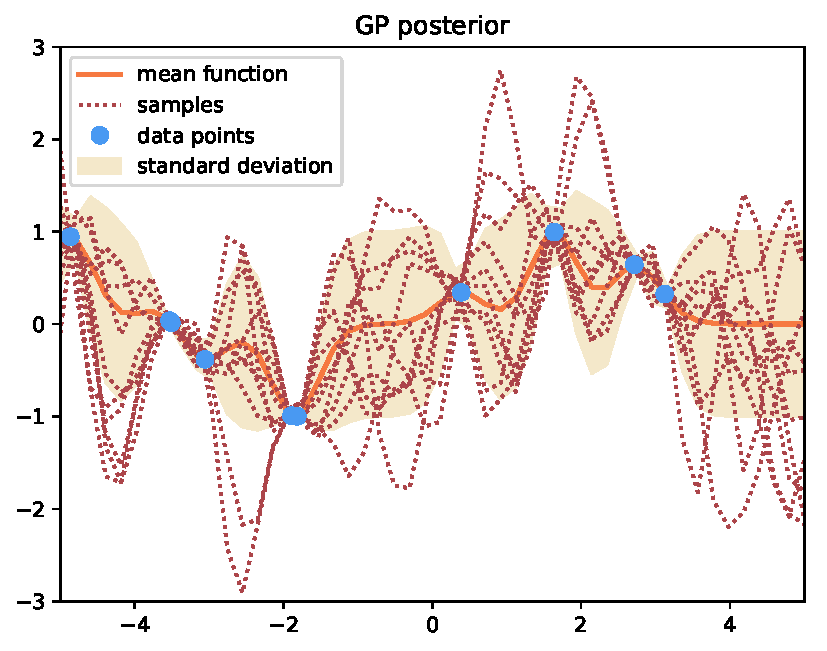
\includegraphics[width=0.9\textwidth,height=0.16\textheight]{images/post.pdf}
		\caption{A Gaussian process is a distribution over the space of functions that describe data (blue).}
	\end{minipage}
\end{figure}



\subsection{Leveraging Attributes}
While decision trees are suitable for tabular data, applying them to image data is not trivial. Images are parameterized by pixels rather than attributes, so attributes have to be provided as side information. Ideally, those attributes should correspond to features that characterize classes found in the image data. Therefore, a popular way of acquiring side information is through human labeling of data according to characteristics suggested by domain experts. \citet{WahCUB_200_2011} let users label different kinds of bird species according to attributes and collect them in the CUB dataset. Another dataset containing attributes as side information is proposed by \citet{8413121}.\\
Attributes can be used to create an interpretable output of a neural network. \citet{akata2013label} propose to learn a linear mapping between feature representations of a neural network and attribute representations.
In other areas, attributes are used as well. \citet{kulkarni2013babytalk} and \citet{ordonez2011im2text} use attributes for image captioning. \citet{lampert2009learning} and \citet{palatucci2009zero} use attributes for zero-shot learning.


\subsection{Multi-agent Communication}
Communication between different agents is a popular technique in reinforcement learning \cite{havrylov2017emergence, lazaridou2018emergence, cao2018emergent, jiang2018learning, das2019tarmac}. \citet{foerster2016learning} propose to let one agent send messages containing categorical symbols that can be used by a second agent to solve a problem. Multi-agent communication has also been applied to create interpretable outputs by \citet{rodriguez2019modeling} who take into account that different agents may have different understandings of concepts. Communication between two agents is also the basis for learning in the RDTC.


\section{Uncertainty in Machine Learning}
Uncertainty is an important factor in human decision making. Modeling uncertainty in machine learning methods is useful for ensuring responsible decision making of algorithms and allows a user to build trust in these models. Uncertainty can arise from data. This is called aleatoric uncertainty. It compromises all kinds of noise inherent to the data. If this noise is static (i.e. limited precision of a sensor) it is called homoscedastic uncertainty. If noise is not static (i.e. occlusions in an image) the uncertainty is called heteroscedastic uncertainty \cite{kwon2020uncertainty}.\\
On the other hand, a model can also be uncertain about its parameters. This uncertainty is called epistemic uncertainty and is high if a model has seen few data. By giving it more data, it can be reduced. Those two kinds of uncertainty are displayed for a computer vision task in Figure \ref{fig:uncertainty_example}.
% image that shows the heteroscedastic and epistemic uncertainty
\begin{figure}
	\centering
	\includegraphics[width=0.9\textwidth]{images/uncertainty_example.png} 
	\caption{Areas with high aleatoric uncertainty are marked red. These are mostly due to occlusions in the image. The area in purple is due to high epistemic uncertainty since the model has never seen a boat before. It misclassifies it as a car but is uncertain about this classification.}
	\label{fig:uncertainty_example}
\end{figure}


\subsection{Bayesian Inference}
Applying Bayes' theorem to update prior beliefs as more data becomes available is called Bayesian inference \cite{box2011bayesian}. This is useful when only partial data is available but a posterior has to be computed already. This posterior can then incrementally be improved, according to new data.
 Bayes' theorem was introduced by \citet{bayes1763lii} and is stated as
\begin{align}\label{eq:bayestheorem}
	p(a|b) = \frac{p(b|a) \cdot p(a)}{p(b)}.
\end{align}
Intuitively put, it computes the posterior conditional probability of a random variable $a$ given the likelihood of $b$ being true given $a$ is true: $p(b|a)$, a prior believe $p(a)$, and a marginalization term $p(b)$. Methods of Bayesian inference are popular in different fields of science, such as neurology, psychology, medicine, epidemiology, geography and machine learning \cite{friston2002classical,wagenmakers2018bayesian,koch2006bayesian,parmigiani2002modeling,didelot2014bayesian,ghahramani2015probabilistic}. They can be used to incorporate prior knowledge, multiple sources of evidence, or, in general, construct large joint probability density functions \cite{Spiegelhalter:2009}.


\subsection{Variational Inference}\label{sec:vi}
Methods of variational inference are used when intractable integrals are encountered in Bayesian inference \cite{jordan1999introduction}. To retrieve the posterior in Equation \ref{eq:bayestheorem}, the denominator has to compute the probability for all possible $a$. The posterior becomes intractable, when $a$ can take many possible values.\\
Suppose, we want to find the predictive posterior $p(y^*|x^*, X,Y)$ for some datapoint $x^*$, we need to compute
\begin{align*}
p(y^*|x^*, X,Y) = \int p(y^*|x^*, w)p(w|X,Y)dw.
\end{align*}
As we have seen, the true posterior over model parameters, given data $p(w|X,Y)$ is not trivial to find and is often intractable in practice. Therefore, an approximate distribution $q_{\theta}(w)$, with optimizable parameters $\theta$ is used. Ideally, $q_{\theta}(w)$ should be similar to the true posterior. To compare the two distributions, we use the Kullback–Leibler divergence (KL-divergence).
\begin{align*}
KL(q_{\theta}(w)|p(w|X,Y)).
\end{align*}
The KL-divergence tells us how different the approximate distribution is from the true posterior \cite{Joyce2011}. Thus, we minimize the KL-divergence between the two.\\
Given an approximate distribution, the predictive posterior can be written as
\begin{align*}
p(y^*|x^*) \approx \int p(y^*|x^*, w)q_{\theta}(w)dw.
\end{align*}
To find the variational distribution $q_{\theta}^*(w)$ with the optimal set of parameters, we have the objective
\begin{align*}
\mathcal{L}_{VI} := \int q_{\theta}(w) log\;p(Y|X, w)dw - KL(q_{\theta}(w)|p(w))
\end{align*}
that is optimized with respect to parameters $\theta$. Here, $p(w)$ is a prior that is often assumed to be a standard Gaussian. According to \citet{bishop2006pattern}, maximizing the log evidence lower bound is equivalent to minimizing the KL-divergence but does not require having access to the true posterior $p(w)$. This effectively leaves us with an optimization task where we need to compute derivatives instead of integrals. This, in turn, allows us to apply powerful automatic differentiation tools, such as deep learning frameworks.



\subsection{Gaussian Processes}\label{sec:gp}
 %TODO citations
Gaussian processes (GP) are a powerful, generative model that can be applied to a variety of machine learning tasks \cite{mackay1998introduction}. They build on the notion that data can be described by (possibly infinitely) many functions. GP's assign probabilities to functions that describe given data. Starting with a prior distribution over the space of functions, a GP eventually returns a posterior over this space, given new data. Of course, distributions over functions are somewhat hard to define. Therefore, we will view a function $f(x)$ as a vector where the $x$ denotes the index that will retrieve the function value at this point. Now, a GP is a joint normal distribution over the points of this vector, defined by a mean function $\mu(x)$ and a covariance function $\Sigma(x)$ with $\Sigma(x) = \Sigma_{ij} = k(x_i,x_j)$. The kernel function $k$ has to return a positive definite matrix and should return a high output for similar $x_i$ and $x_j$.\\
GP's thus view each $x_i$ as a random variable, that is dependent on all other $x_j\neq x_i$.\\
To perform inference in a GP, one simply takes the conditional probability density distribution (PDF) of a given $x_i$ conditioned on all other $x_j\neq x_i$. Since Gaussian distributions are closed under conditioning, the resulting PDF is Gaussian as well.\\
To retrieve a meaningful posterior from a GP, it has to be trained in a supervised fashion. We will describe the key steps in Algorithm~\ref{alg:gpcode}.


\begin{algorithm}
	\caption{Inference in a GP}
	\label{alg:gpcode}
	\begin{algorithmic}
\STATE -create a prior-
\STATE $x_{test}$= $\lbrace x_n \rbrace$
\STATE $K_{prior}$ = kernel($x_{test}$, $x_{test}$, $w$)
\STATE $L_{prior}$ = cholesky\_decomposition($K_{prior}$)
\STATE $f_{prior}$ = $L_{prior} \cdot \mathcal{N}(dim=(n, num\_samples);0,1)$
\STATE
\STATE -take new data into account and compute new posterior-
\STATE $x_{train}$, $y_{train}$ = training data
\STATE $K$ = kernel($x$, $x$, $w$)
\STATE $L$ = cholesky\_decomposition($K$)
\STATE $K_s$ = kernel($x_{train}$, $x_{test}$, $w$)
\STATE $L_k$ = solve($L$, $K_s$)
\STATE $\mu$ = $L_k^T \cdot$ solve($L, y_{train}$)
\STATE
\STATE -draw samples from posterior-
\STATE $L$ = cholesky\_decomposition($K_{ss}$ - $L_k^T \cdot L_k$)
\STATE $f_{posterior}$ = $\mu$ + $L \cdot \mathcal{N}(dim=(n, num\_samples);0,1)$
\STATE - prediction at test point $x_i$ is now the sample's value at position $i$-
	\end{algorithmic}
\end{algorithm}


\subsection{Dropout Variational Inference} %TODO maybe why softmax does not yield 
%Alternative title: Modeling Uncertainty in Neural Networks
Deep neural networks (DNN) are applied in safety-critical processes where information about a model's uncertainty is of crucial importance \cite{najafabadi2015deep,krzywinski2013importance}. Standard DNN's however do not yield uncertainty information. Bayesian neural networks (BNN) are an architecture that can model uncertainty reliably \cite{mullachery2018bayesian}. However, they require modeling a probability density function over each parameter which causes high computational costs. A method using variance arising from dropout has been proposed by \citet{gal2016dropout} who proofed that dropout in neural networks is equal to Monte-Carlo integration in GP's and thus can be used to model epistemic uncertainty.\\
With a GP, we want to find a posterior distribution over function that explains given data. We can view a finite model like a neural network as an approximation to a GP \cite{damianou2013deep}. Thus, by optimizing a model, we minimize the Kullbach-Leibler (KL) divergence between our finite model and the corresponding GP \cite{gal2016dropout}. In practice, however, the GP's posterior often requires computing intractable integrals. To alleviate this, methods of variational inference, such as Monte-Carlo integration are applied. Monte-Carlo integration in a GP corresponds to averaging forward passes in a dropout neural net. According to \citet{gal2016dropout}, the resulting variance can be viewed as the model's uncertainty.
\\
Additionally, \citet{kendall2017uncertainties} propose to combine aleatoric and epistemic uncertainty in a unified approach. They estimate epistemic uncertainty with dropout and learn to predict high aleatoric uncertainty for falsely classified examples.
For classification tasks, this has been simplified by \citet{kwon2020uncertainty}. Instead of learning uncertainty, they model aleatoric based on the distribution of softmax output values.





\chapter{Uncertain Recurrent Decision Tree Classifier} % aka Methods aka Architecture
The RDTC model, proposed by \citet{alaniz2019explainable}, consists of two communicating agents; a Recurrent Decision Tree agent (RDT) and an Attribute-based Learner agent (AbL). Their common goal is to solve a classification task through communication. The RDT has no direct access to the data and can only ask questions regarding attributes. Given answers by the AbL, it can then store the answers in a memory and thus incrementally build a decision tree that is used for the final classification. The learned decision tree allows introspection.\\
Based on their work, we propose a model, where the AbL is aware of and able to express its uncertainty for given attributes (Figure \ref{fig:uncertainRDTC}). We use this uncertainty information by either preventing the RDT from using uncertain attributes or by allowing the AbL to answer with 'I don't know' additionally to the options 'Yes' or 'No'\footnote{A Pytorch implementation of our model can be found at \url{github.com/wastedsummer/urdtc}}.



\begin{figure}
	\centering
	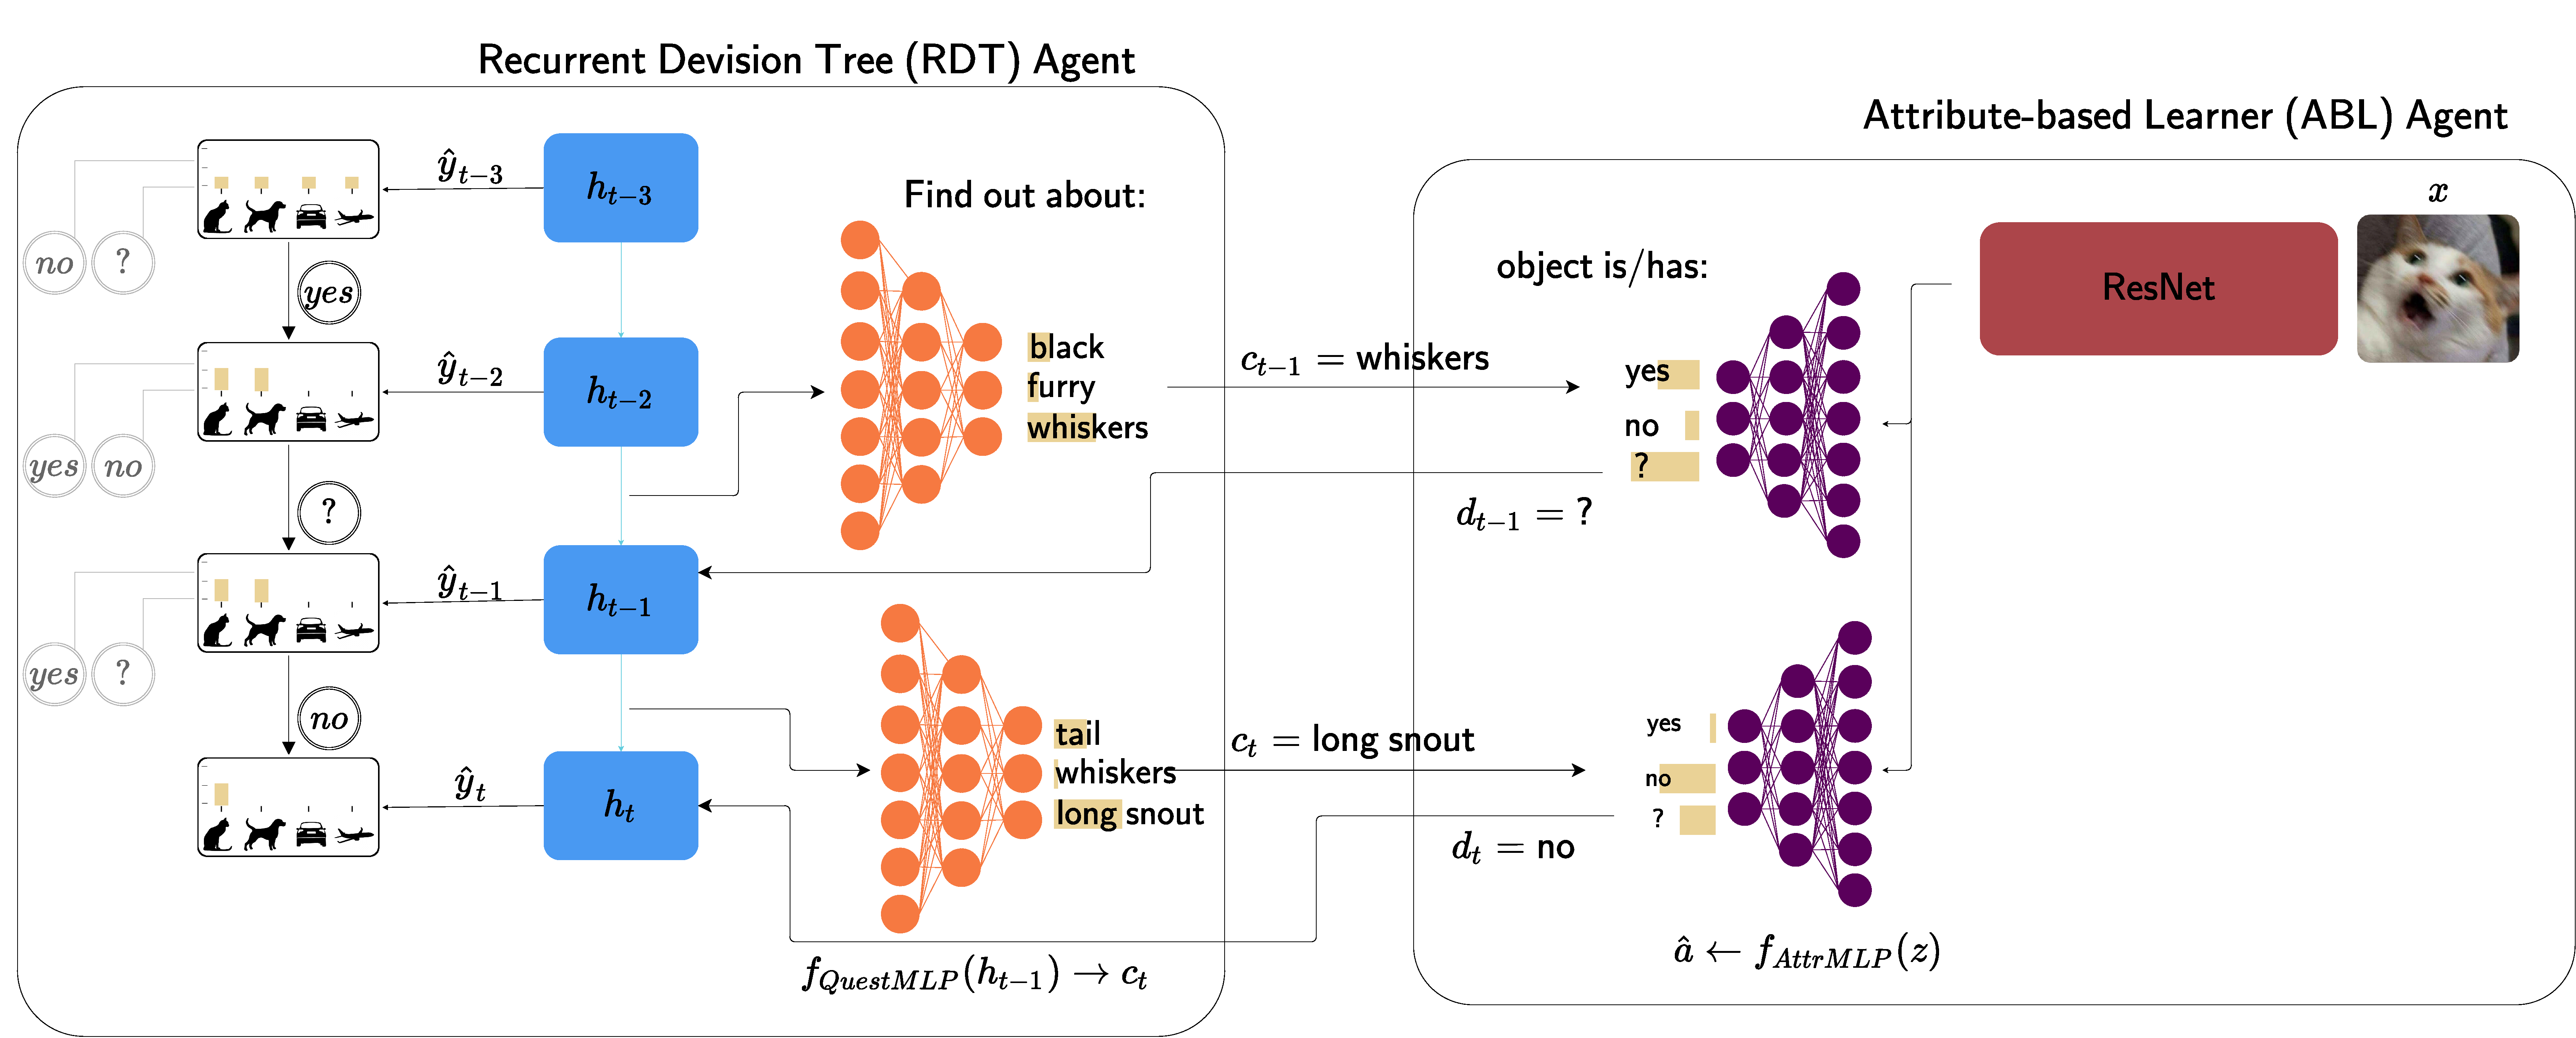
\includegraphics[width=1\textwidth]{images/uncertaintRDTC.pdf} 
	\caption{The RDT asks questions about presence, absence or uncertainty of attributes. The answers, given by the AbL are used by the RDT agent to make a classification each iteration.}
	\label{fig:uncertainRDTC}
\end{figure}

\section{The RDTC Model} 
Before we introduce our modifications to the RDTC model, we will give a detailed explanation of its architecture, learning algorithm, and how the two agents communicate.

%TODO intro
\subsection{Communication}
The two agents communicate with each other through discrete messages. For a given image $x$, the AbL returns a an answer $\hat{a}$ that is a tensor with binary values with shape $\text{number of attributes} \times \text{decision size}$. The intention behind using only binary values in the AbL's answer is increased interpretability. Each row in this tensor indicates the presence/absence of an attribute and the columns correspond to the decision options 'Yes' or 'No'. Strictly speaking, the AbL thus answers all possible questions the RDT can ask, in advance to any questions.\\
The RDT is then able to ask questions by posing an index $c_t$. By accessing the AbL's answer at this index it receives answer $d_t = \hat{a}[d_t]$. This information is then used to build an internal decision tree, used for a classification output and to come up with a new question. In the following, we will go over each agent in more detail and explain how this model is trained.


\subsection{Attribute-based Learner}
The AbL agent is a vision model, consisting of a CNN and an MLP. The CNN learns image features and the MLP ($f_{AttributeMLP}$) learns a mapping from features to human-annotated attributes (if available). For all experiments, we use a ResNet \cite{he2016deep} to extract features. For a given image $x$, the CNN extracts feature vector $z$. This is passed to the $f_{AttributeMLP}$ and the resulting vector of logits is put through a softmax with temperature (TempSoftmax in Equation~\ref{eq:tempsoftmax}). The output is a tensor $p(\hat{a}|z)$ with shape $\text{number attributes} \times \text{decision size}$. This corresponds to a probability distribution over the decision option for each attribute. To get an interpretable, binary response, in the forward pass, the result of the TempSoftmax is put through an arg max function. This is, however, not differentiable. In the backward pass, it is therefore replaced by the identity function. Thus, the final response of the AbL agent for a given image $x$ is $\hat{a} = argmax(p(\hat{a}|z))$. The RDT agent can then access answers for specific attributes through indexing.

\begin{align}\label{eq:tempsoftmax}
&TempSoftmax(log\;\pi) = \frac{exp((log\;\pi_i)/\tau)}{\sum_{j=1}^{K}exp((log\;\pi_j)/\tau)} = d_t,\\
\text{ where }
log\;\pi &\text{ are the logit values for either 'Yes', or 'No' per attribute.}%&=log\;p(c_t|h_{t-1})\text{ , and thus:}
%c_t &= GumbelSoftmax(log\;p(c_t|h_{t-1})).
\end{align}


\subsection{Recurrent Decision Tree}
The RDT agent consists of several models. At its core lies a LSTM. This recurrent model allows the RDT to come up with new questions, based on its hidden state $h_{t-1}$ from the previous (or initial) communication step.\\
The MLP $f_{QuestMLP}$ is responsible for thinking of new questions by returning an index that can be used to access attribute information in the response from $f_{AttributeMLP}$. The output of $f_{QuestMLP}$ are logit values $log\;p(c_t|h_{t-1})$ over possible indices $c_t \ in \lbrace 1,2,...,|A| \rbrace$, where $|A|$ is the number of available attributes. To get an actual index, the final output needs to be discrete. Thus we need to turn the logit values into a categorical distribution and sample from it. This is done via the Gumbel softmax function \cite{jang2016categorical}:
\begin{align}
		GumbelSoftmax(log\;\pi) &= \frac{exp((log\;\pi_i + g_i)/\tau)}{\sum_{j=1}^{K}exp((log\;\pi_j + g_j)/\tau)}\text{ , where}\\
			log\;\pi &=log\;p(c_t|h_{t-1})\text{ , and thus:}\\
			c_t &= GumbelSoftmax(log\;p(c_t|h_{t-1})).
\end{align}
where for $\tau \rightarrow 0$, the distribution approaches a one-hot vector with a $1$ at the maximum of the categorical distribution and $0$ everywhere else, turning it into a sample, effectively.\\
The resulting tensor $c_t$ then can be used to index $\hat{a}$. The response is $d_t$ which indicates absence, presence (or other possible answers) of the attribute at index $c_t$. Question $c_t$ and answer $d_t$ then update the explicit memory $\mathcal{M}^{(t)} = \mathcal{M}^{(t-1)} \oplus (c_t, d_t)$. Note that during test time, rather than sampling $c_t$, the index with the highest probability is chosen through an argmax because it does not need to be differentiable.\\
The explicit memory $\mathcal{M}^{(t)}$, $c_t$, $d_t$ and the LSTM's last hidden state $h_{t-1}$ are then used to compute the current hidden state $h_t$, which is then, in turn, used by the $f_{QuestMLP}$ to pose a new question.\\
The explicit memory $\mathcal{M}^{(t)}$ is also the basis for the class prediction. An additional MLP, the $f_{ClassMLP}$ returns class probabilities $\hat{y}_t$ based on  $\mathcal{M}^{(t)}$ for every communication step:
\begin{align}
	\hat{y}_t = f_{ClassMLP( \mathcal{M}^{(t)})}.
\end{align} The classification is the final output of the model and is used to calculate a loss that can be optimized.


\subsection{Learning}
Ideally, the model should come to a classification in as few communication steps as possible. A tree resulting from few communication steps is shallow and easier to interpret. To keep the model from using deep trees, the classification loss is divided by the number of time steps (communication steps):
\begin{align}
	\mathcal{L} = \frac{1}{T} \sum_{t=1}^{T}\mathcal{L}_{CE}(y, \hat{y}_t) = - \frac{1}{T}\sum_{t=1}^{T}\sum_{i}y_i \cdot log\;\hat{y}_{t,i}.
\end{align}
This ensures, that the lower the number of time steps $T$, the lower the whole term, and thus, the lower the loss.\\
Besides the classification loss, an additional attribute loss can be leveraged to encourage learning attributes that correspond to provided human-annotated side information.
\begin{align}
	\mathcal{L} = \frac{1}{T}\sum_{t=1}^{T}\left[(1-\lambda)\mathcal{L}_{CE}(y,\hat{y}_t) + \lambda \mathcal{L}_{CE}(\alpha_{y,c_t},\hat{\alpha}_{c_t}) \right]
\end{align}
How much each loss contributes to the total loss can be determined by hyperparameter $\lambda$.




\section{Introducing Uncertainty}
Uncertainty information is a crucial part of robust vision systems. In safety-critical applications, it could be used to prevent the model from using high-risk strategies by leveraging attributes it is highly uncertain about for its classification. Or, if all attributes are deemed highly uncertain (for example on completely OOD data), the model could decide to consult a human instead of making an overconfident classification.\\
Uncertainty comes either from variance in data (aleatoric uncertainty) or from variance in model parameters (epistemic uncertainty). Thus, there is an inherent relationship between variance and uncertainty.
%To get an intuition of the relationship between uncertainty and variance, let us have look at the basic equation for the variance.
The variance of a random variable, which in our case is the variational predictive distribution $p(\hat{y} | x)$ with $y\sim p(\hat{y} | x)$, is defined as:
\begin{align*}
	Var_q(p(\hat{y} | x)) &= \mathbb{E}_q \left[ (y-\mathbb{E}\left[ y\right])^2 \right]\\
	&= \mathbb{E}_q \left[yy^T\right]  - \mathbb{E}_q\left[y\right]\mathbb{E}_q\left[y\right]^T.
\end{align*}
To decompose the term into variance arising from data and variance from the model $q$ itself, according to \citet{kwon2020uncertainty}, we can write it as:
\begin{align*}
Var_q(p(\hat{y} | x)) &= \mathbb{E}_q \left[yy^T\right]  - \mathbb{E}_q\left[y\right]\mathbb{E}_q\left[y\right]^T\\
	&\underbrace{=\int_{\Omega}\left[ diag (\mathbb{E}_{p(\hat{y}|x,w)}[\hat{y}]) -\mathbb{E}_{p(\hat{y}|x,w)}[\hat{y}] \cdot \mathbb{E}_{p(\hat{y}|x,w)}[\hat{y}] \right]q_{\theta}(w)dw}_{aleatoric}\\
	&+\underbrace{\int_{\Omega}\left[ \mathbb{E}_{p(\hat{y}|x,w)}[\hat{y}] - \mathbb{E}_{q_{\theta}(\hat{y}|x,w)}[\hat{y}] \right] \left[ \mathbb{E}_{p(\hat{y}|x,w)}[\hat{y}] - \mathbb{E}_{q_{\theta}(\hat{y}|x,w)}[\hat{y}] \right]^T}_{epistemic}.
\end{align*}




\subsection{Estimating Epistemic Uncertainty with Dropout Neural Networks}\label{sec:dropoutuncertainty}
Epistemic uncertainty corresponds to the variance of a model's parameters.
In a traditional dropout neural network, there is no random dropping out of neurons at test time, and weights are fixed. This would result in no variance of model outputs for multiple forward passes given the same input. However, dropping out neurons in a random manner results in an inherent variance of model parameters. \citet{gal2016dropout} proof that this variance corresponds to epistemic uncertainty. In the following, we will go through their proof.\\
The key idea is that a dropout neural net is equivalent to an approximation of a Gaussian process using variational inference. To randomly dropout neurons, we sample binary values that are either $0$ or $1$ for every neuron. The sampled value is then multiplied with the neuron's value.
In the following, the dropout neural network's layers are denoted by $L$, the respective weight matrices are denoted by $W_{l \in L}$, the bias vectors by $b_l$, the network output, given datapoint $x_i \in X$ with size $N$ by $\hat{y}_i$, and the true value by $y_i \in Y$. The objective of the network is to minimize a given loss function $E(y_i, \hat{y}_i)$. Additionally, a weighted regularization term can be added to the loss function. A popular technique is to use $L_2$ regularization, weighted by a weight decay term $\lambda$. The final resulting loss term is:
\begin{align*}
\mathcal{L}_{dropout} := \frac{1}{N}\sum_{i=1}^{N}E(y_i, \hat{y}_i) + \lambda \sum_{l=1}^{L}(||W_l||^2_2 + ||b_l||^2_2).
\end{align*}
For the special case of a single hidden layer dropout network (which we will consider for simplicity), we can state this objective as
\begin{align}\label{eq:dropout}
\mathcal{L}_{dropout} := \frac{1}{N}\sum_{i=1}^{N}E(y_i, \hat{y}_i) + \lambda (||W_1||^2_2 + ||W_2||^2_2+ ||b||^2_2),
\end{align} where $W_1$ is the weight matrix connecting the input to the hidden layer, and $W_2$ connecting the hidden to the output layer, and $b$ the connection between a bias neuron and the hidden layer's neurons.\\
Let us take a step back to a very general point of view. A problem we typically encounter in machine learning is how to predict a function value $y^*$ from a datapoint $x^*$. In Bayesian terms, we want to find the predictive posterior
\begin{align}\label{eq:pred_post}
 p(y^*|x^*, X,Y) = \int p(y^*|x^*, w)p(w|X,Y)dw,
\end{align}
where $w$ is a set of adjustable parameters. To model our function of interest well, we need to find optimal values for $w$. If we break down Equation \ref{eq:pred_post} further, we get
\begin{align}
p(y^*|x^*, X,Y) = \int \underbrace{p(y^*|x^*,w)}_{\mathcal{N}(\underbrace{y;\hat{y}(x,w)}_{\hat{y}(x, w=\lbrace W_1, W_2,...,W_n\rbrace)},\tau^{-1}\mathbf{I}_D)} \cdot \hspace{15pt}\underbrace{p(w|X,Y)}_{intractable}dw,
\end{align}
where we see that the posterior over $w$, given data is intractable, which is why we approximate it with variational distribution $q_{\theta}(w)$. We want this distribution to mimic the true posterior closely, so we want to find
\begin{align*}
	argmin_{\theta} KL(q_{\theta}(w)|p(w|X,Y)).
\end{align*}
As we have seen in Section \ref{sec:vi}, this would require access to the true posterior, which we cannot compute. Therefore, we maximize the log evidence lower bound
\begin{align*}
\mathcal{L}_{VI} := \int q_{\theta}(w) log p (Y|X, w)dw - KL(q_{\theta}(w)||p(w))
\end{align*}
and assume $p(w)$ to be a standard Gaussian. As discussed in Section \ref{sec:vi}, we effectively turn computing integrals into an optimization problem, where we need to compute derivatives. Using the optimized variational distribution $q_{\theta}^*(w)$, we can compute an approximate predictive posterior 
\begin{align*}
q_{\theta}(y^*|x^*) = \int p(y^*|x^*, w)q_{\theta}^*(w)dw
\end{align*}
for a given datapoint $x^*$. This in turn can be approximated with
\begin{align*}
q_{\theta}(y^*|x^*) = \sum_{t=1}^{T}p(y^*|x^*, w_t)
\end{align*}
where each $w_t$ is a sample from our variational distribution $p_{\theta}^*(w)$.
\\
Now, in Gaussian processes, as discussed in Section \ref{sec:gp}, we need a covariance function of the form 
\begin{align*}
K(x,y) = \int \mathcal{N}(w;0, l^{-2} I_Q)p(b)\sigma(w^Tx+b)]\sigma(w^Ty +b)dwdb
\end{align*}
to retrieve a covariance matrix. To avoid computing integrals, this covariance function can be approximated with
\begin{align*}
	\hat{K}(x,y) = \frac{1}{K} \sum_{K}^{k=1} \sigma(w^T_k x + b_k)\sigma(w^T_k y + b_k)
\end{align*}
where $w_k$ is sampled from $\mathcal{N}(0, l^{-2}I_Q)$ and $b_k$ from $p(b)$. This is called Monte-Carlo integration \cite{metropolis1949monte}.\\
We get the following predictive posterior for our GP:
\begin{align*}
w_k \sim \mathcal{N}(0, l^{-2}I_Q), w_d \sim \mathcal{N}(0, l^{-2} I_K), b_k \sim p(b)\\
W_1 = \left[ w_k \right]^{K}_{k=1}, W_2 = \left[ w_d \right]^D_{d=1}, b = \left[ b_k \right]^K_{k=1}, w = \lbrace W_1, W_2, b \rbrace\\
p(y^*|x^*, w) = \mathcal{N} \left( y^*; \sqrt{\frac{1}{K}\sigma(x^* W_1 + b)W_2, \tau^{-1}I_N}\right),\\
\text{and finally:}\hspace{160pt}\\
p(y^*|x^*, X,Y) = \int p(y^*|x^*, w)p(w|X,Y)dw.
\end{align*}
%TODO note that this is for normal GP and single hidden layer dropout net
We use $q_{\theta}(w) = q_{\theta}(W_1)q_{\theta}(W_2)q_{\theta}(b)$ as an approximation to $p(w|X,Y)$, where
\begin{align*}\label{eq:gaussian_mixture}
q_{\theta}(W_1) = \Pi q_{\theta}(w_q), \text{ and } q_{\theta}(w_q) = p_1\mathcal{N}(m_q, s^2, I_K) + (1-p_1) \mathcal{N}(0, s^2, I_K),\\
\text{ with } p_1 \text{ as a probability }\in \left[ 0, 1\right], s > 0, \text{ and }M_1 = \left[ m_q \right]^Q_{q=1} \in \mathbb{R}^{K\times D}
\end{align*}
We eventually want to recover a dropout neural network (as specified in Equation~\ref{eq:dropout}) from our GP. In our dropout network, we rely on sampling from a Bernoulli random variable. In our GP, we, so far, sample from a mixture of Gaussian distributions. We cannot change this, because the KL-divergence between a discrete distribution (i.e. Bernoulli) and a continuous distribution (i.e. Gaussian) is not defined. Therefore, we will make two assumptions about the Gaussian mixture in Equation~\ref{eq:gaussian_mixture}.\\
We set $p$ to a fixed value. Also, we want the second term of the sum to be zero. To sample zero from a zero-centered Gaussian distribution with a very high probability, we simply set the standard deviation to a very small value. Small enough so that a device with limited precision will view it as zero and always return zero. These two assumptions leave us with a Gaussian distribution that resembles a Bernoulli distribution. Thus, we are effectively sampling from a Bernoulli random variable in our GP, with a still defined KL-divergence. We get
\begin{align*}
\mathcal{N}_{GP-MC} \approx log p(Y|X, \hat{w}) - \frac{p_1 l^2}{2} ||M_1||^2_2 - \frac{p_2 l^2}{2}||M_2||^2_2 - \frac{l^2}{2}||m||^2_2 \text{, with } \hat{w} \sim q_{\theta}(w)
\end{align*}
as approximated log evidence lower bound.
% here, the maximizing variational parameters are the same as in the ELBO specified, above
To recover the dropout objective from Equation \ref{eq:dropout}, we can scale it by a constant $\frac{1}{N \tau}$.
\begin{align*}
\mathcal{L}_{GP_MC} \propto  - \frac{1}{2N} \sum_{n=1}^N ||y_n - \hat{y}_n||^2_2 -  \frac{p_1 l^2}{2N\tau} ||M_1||^2_2 - \frac{p_2 l^2}{2N\tau}||M_2||^2_2 - \frac{l^2}{2N\tau}||m||^2_2
\end{align*}
and set hyperparameters $\tau$ and $l$ to appropriate values. According to \citet{gal2016dropout}, this generalizes to deep GPs and Dropout networks with more than one hidden layer, as well.


\subsection{Retrieving Uncertainty Information}
\begin{figure}
	\centering
	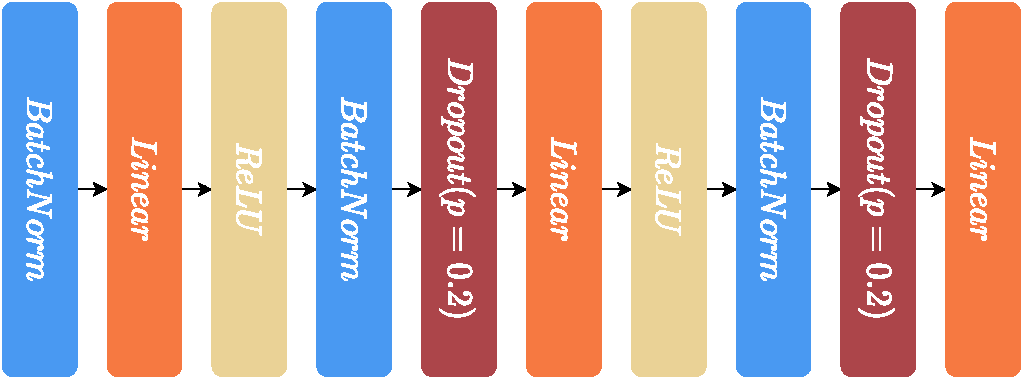
\includegraphics[width=0.9\textwidth]{images/f_attrMLP.pdf} 
	\caption{We used both BatchNorm and dropout layers for $f_{attrMLP}$.}
	\label{fig:f_attrMLP}
\end{figure}
The RDTC model does not use dropout layers in the vision model. As we want to keep the ResNet as a feature extractor and be able to estimate uncertainty, we introduce dropout layers to $f_{AttributeMLP}$. We tested different configurations for $f_{AttributeMLP}$ and found that using a combination of dropout and batchnorm layers between fully connected layers and non-linearities worked best. The setup is displayed in Figure~\ref{fig:f_attrMLP}. To retrieve uncertainty information, given the image features $z$ from the ResNet, we do $n$ forward passes and compute the standard deviation of the results. As proofed by \citet{gal2016dropout} and discussed in Section \ref{sec:dropoutuncertainty}, this is equal to approximated epistemic uncertainty. So theoretically, for examples, that are far from the distribution, the model was trained on, it should yield high epistemic uncertainty.\\
After uncertainty estimation, we use two different strategies of making the model aware of its uncertainties. In the first strategy, we replace selection logits from $f_{QuestMLP}$ that are on indices with high uncertainty by $-inf$ so they can not be picked by the Gumbel softmax. We call this strategy 'remove uncertain attributes' (remRDTC). In another strategy, uncertain attributes are denoted with a $1$ in an extended decision tensor. We refer to this strategy as 'extended vocabulary' (extRDTC). In both strategies, an attribute is deemed uncertain if its uncertainty lies above a threshold that is determined by a hyperparameter.


\subsection{Removing Uncertain Attributes}\label{sec:remRDTC}
%\begin{figure}[t!]
%	\centering
%	\begin{minipage}{0.45\textwidth}
%		\centering
%		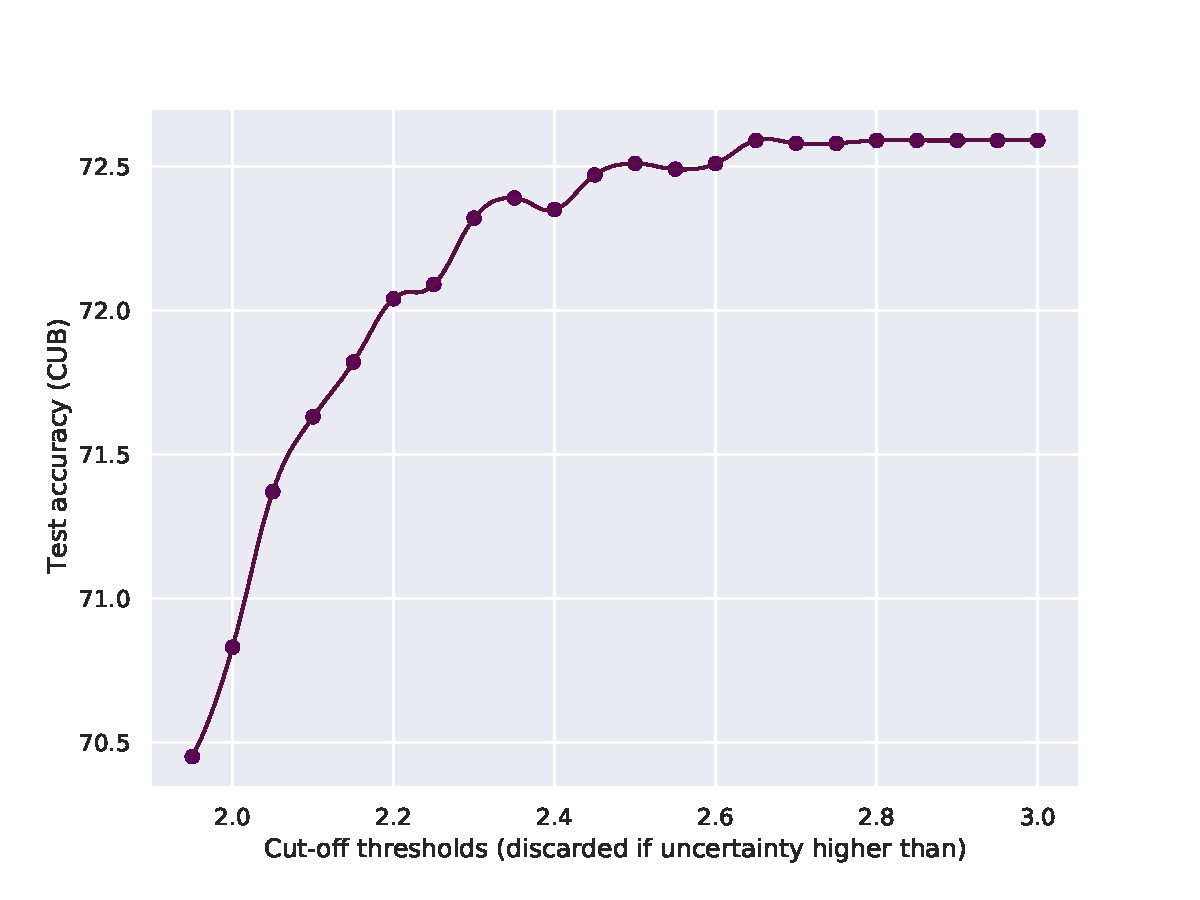
\includegraphics[width=1\textwidth]{images/threshold_accuracy.pdf} 
%		\caption{Test accuracies, when removing uncertain attributes with different thresholds. Note, that here we used a model that was trained for 30 epochs and used max\_iters=20.\\\hspace{40pt}}
%		\label{fig:threshold_accuracies}
%	\end{minipage}\hfill
%	\begin{minipage}{0.45\textwidth}
%		\centering
%		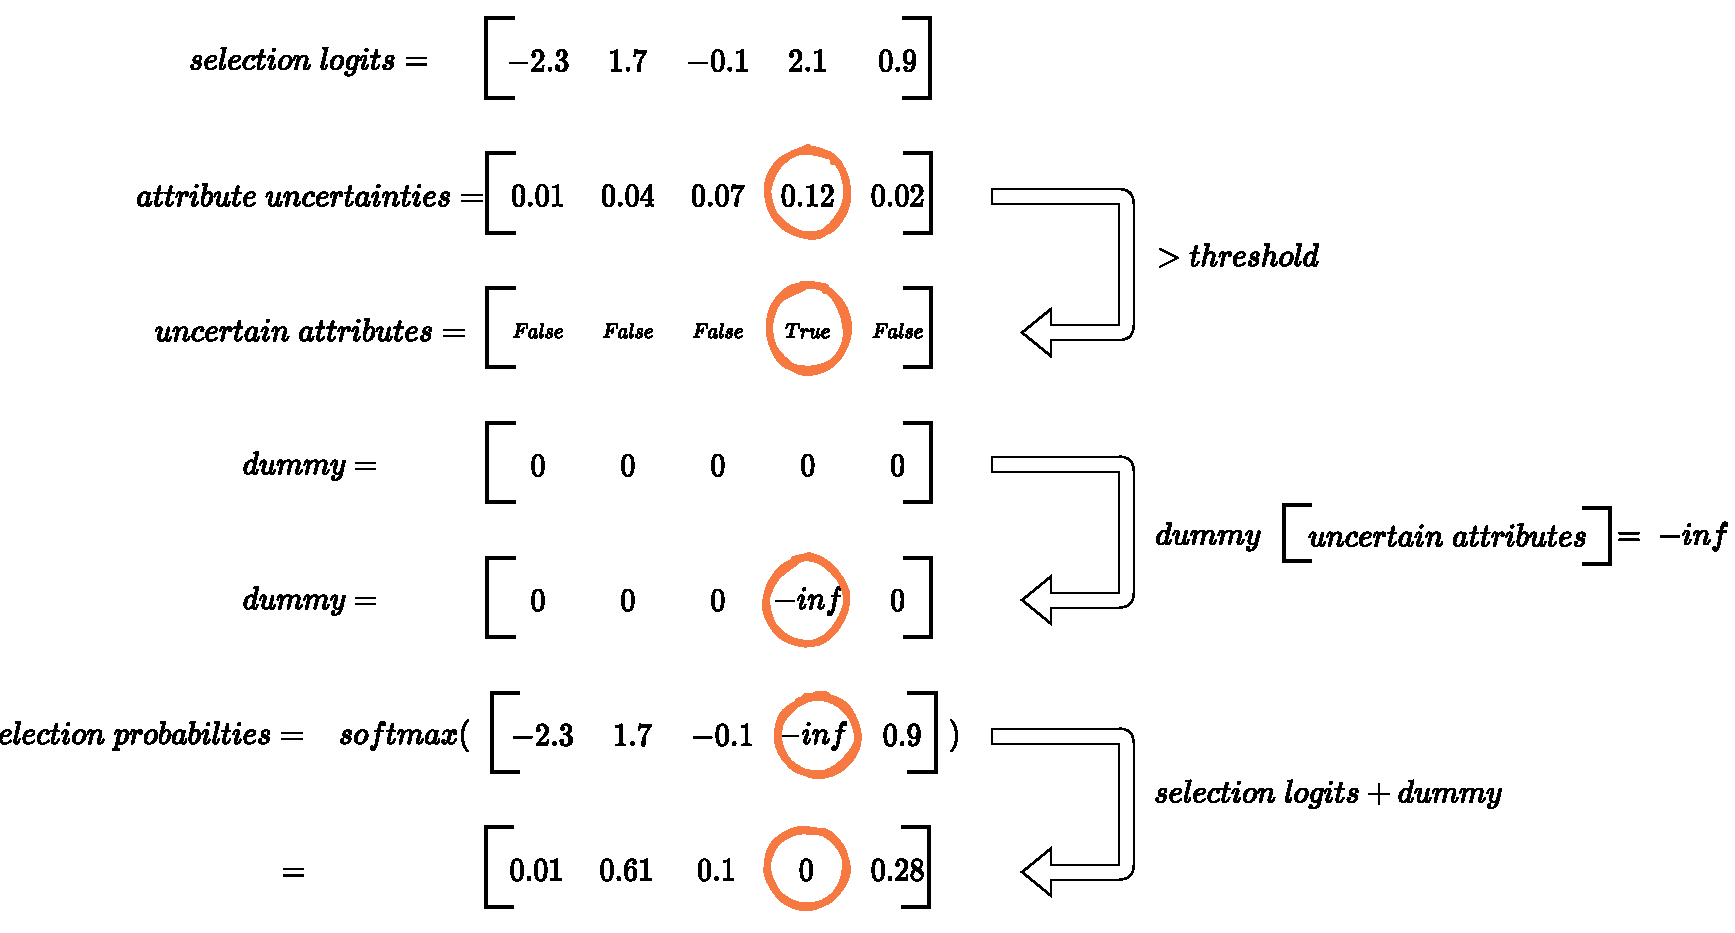
\includegraphics[width=1\textwidth]{images/remove_attrs.pdf}
%		\caption{...}
%		\label{fig:remove_intuition}
%	\end{minipage}
%\end{figure}
\begin{figure}
	\centering
	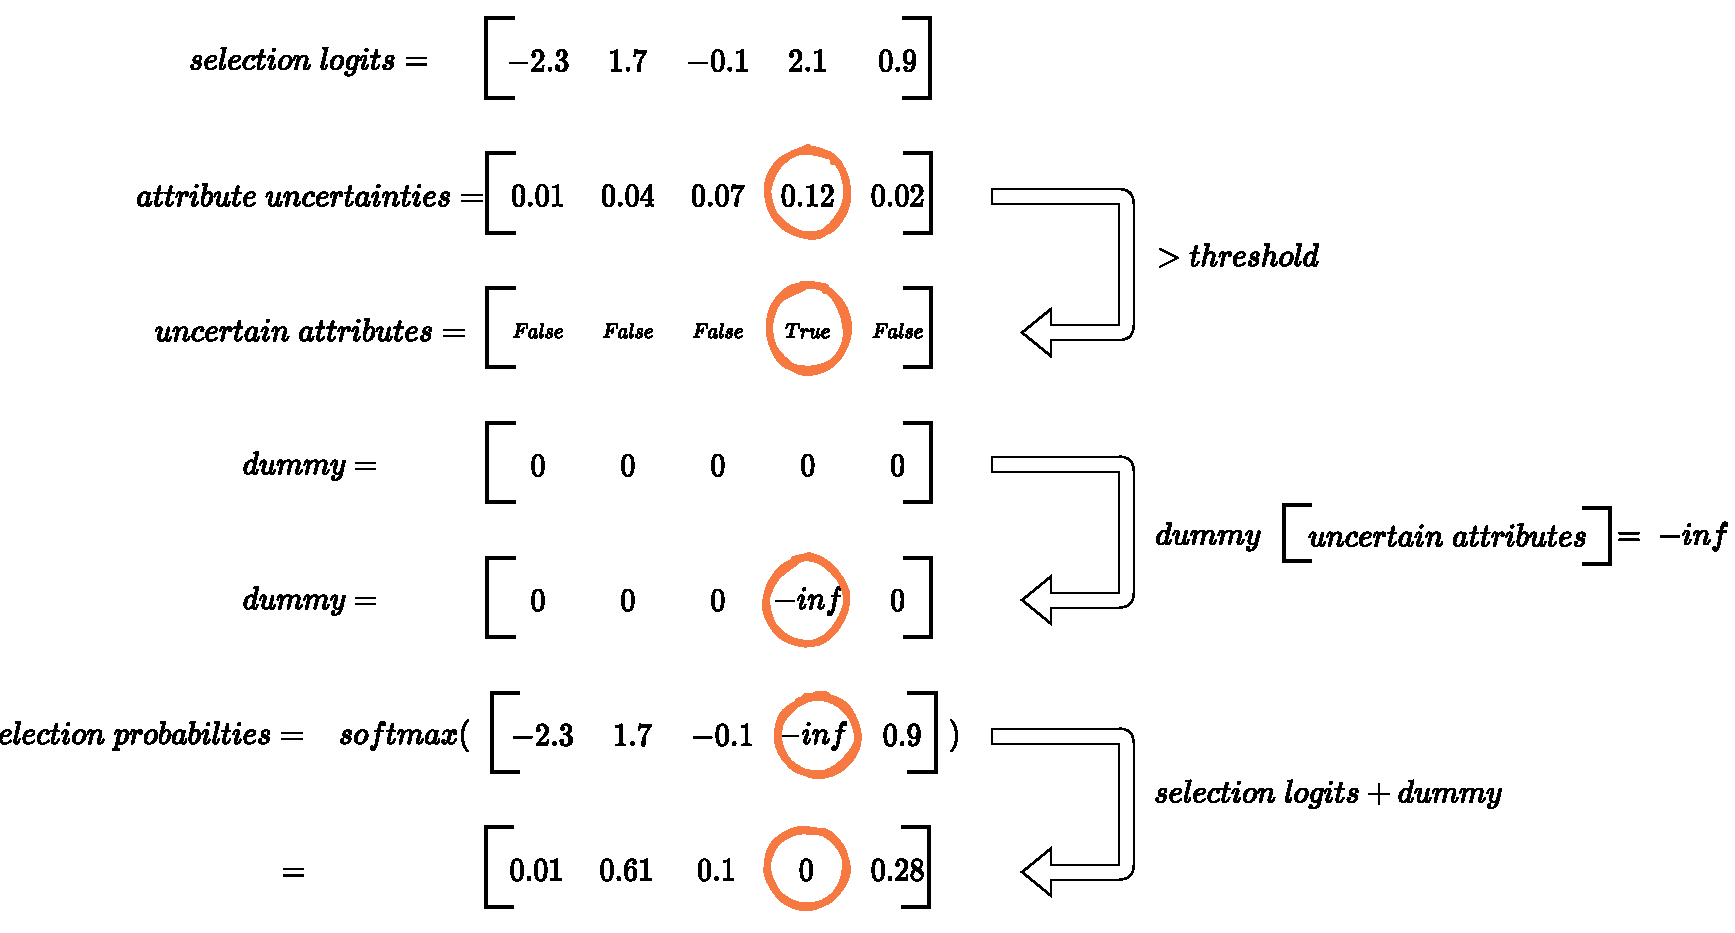
\includegraphics[width=0.9\textwidth]{images/remove_attrs.pdf} 
	\caption{In selection logits (the output from $f_{QuestMLP}$), we replace values at indices where uncertain attributes (orange) are, with a $-inf$ value. This assures that this attribute can never be picked as $c_t$ by the Gumbel softmax.}
	\label{fig:remove_intuition}
\end{figure}


After computing uncertainty for each attribute, in this strategy, we simply manipulate the logits tensor from $f_{QuestMLP}$ so that at each index, where an uncertain attribute is, the selection logit tensor has a $-inf$ value. This ensures that this attribute cannot be picked by the Gumbel softmax. In turn, no uncertain attribute can be picked as an index and therefore cannot be posed as a question to the AbL.\\
To prevent the model from misusing uncertainty information, we have to ensure that the model does not get any gradients from where uncertain attributes are. This is done by detaching all attributes, affiliated with uncertainty from the computational graph. The $n$ forward passes to compute variance are therefore done without adding to the computational graph. Tensors created based on the uncertainty tensor also do not carry gradient information. Thus, in the masked selection tensor (Figure \ref{fig:remove_intuition}) indices of uncertain attributes have a gradient of $0$.

%We tested this strategy both in test-only and in training and testing stage. When using it in the test stage for a model, that was trained regularly (without uncertainty information), the model suffered severe performance drops, displayed in Figure \ref{fig:threshold_accuracies}. Especially, for low cut-off thresholds. It never outperforms a model that keeps all attributes. We hypothesize that this is due to actively removing options from a pool of attributes, that the model is already well adapted to and as shown in Figure \ref{fig:less_attrs} rarely misclassifies despite being uncertain.



\subsection{Extending the Vocabulary}
\begin{figure}[t!]
	\centering
	\begin{minipage}{0.45\textwidth}
		\centering
		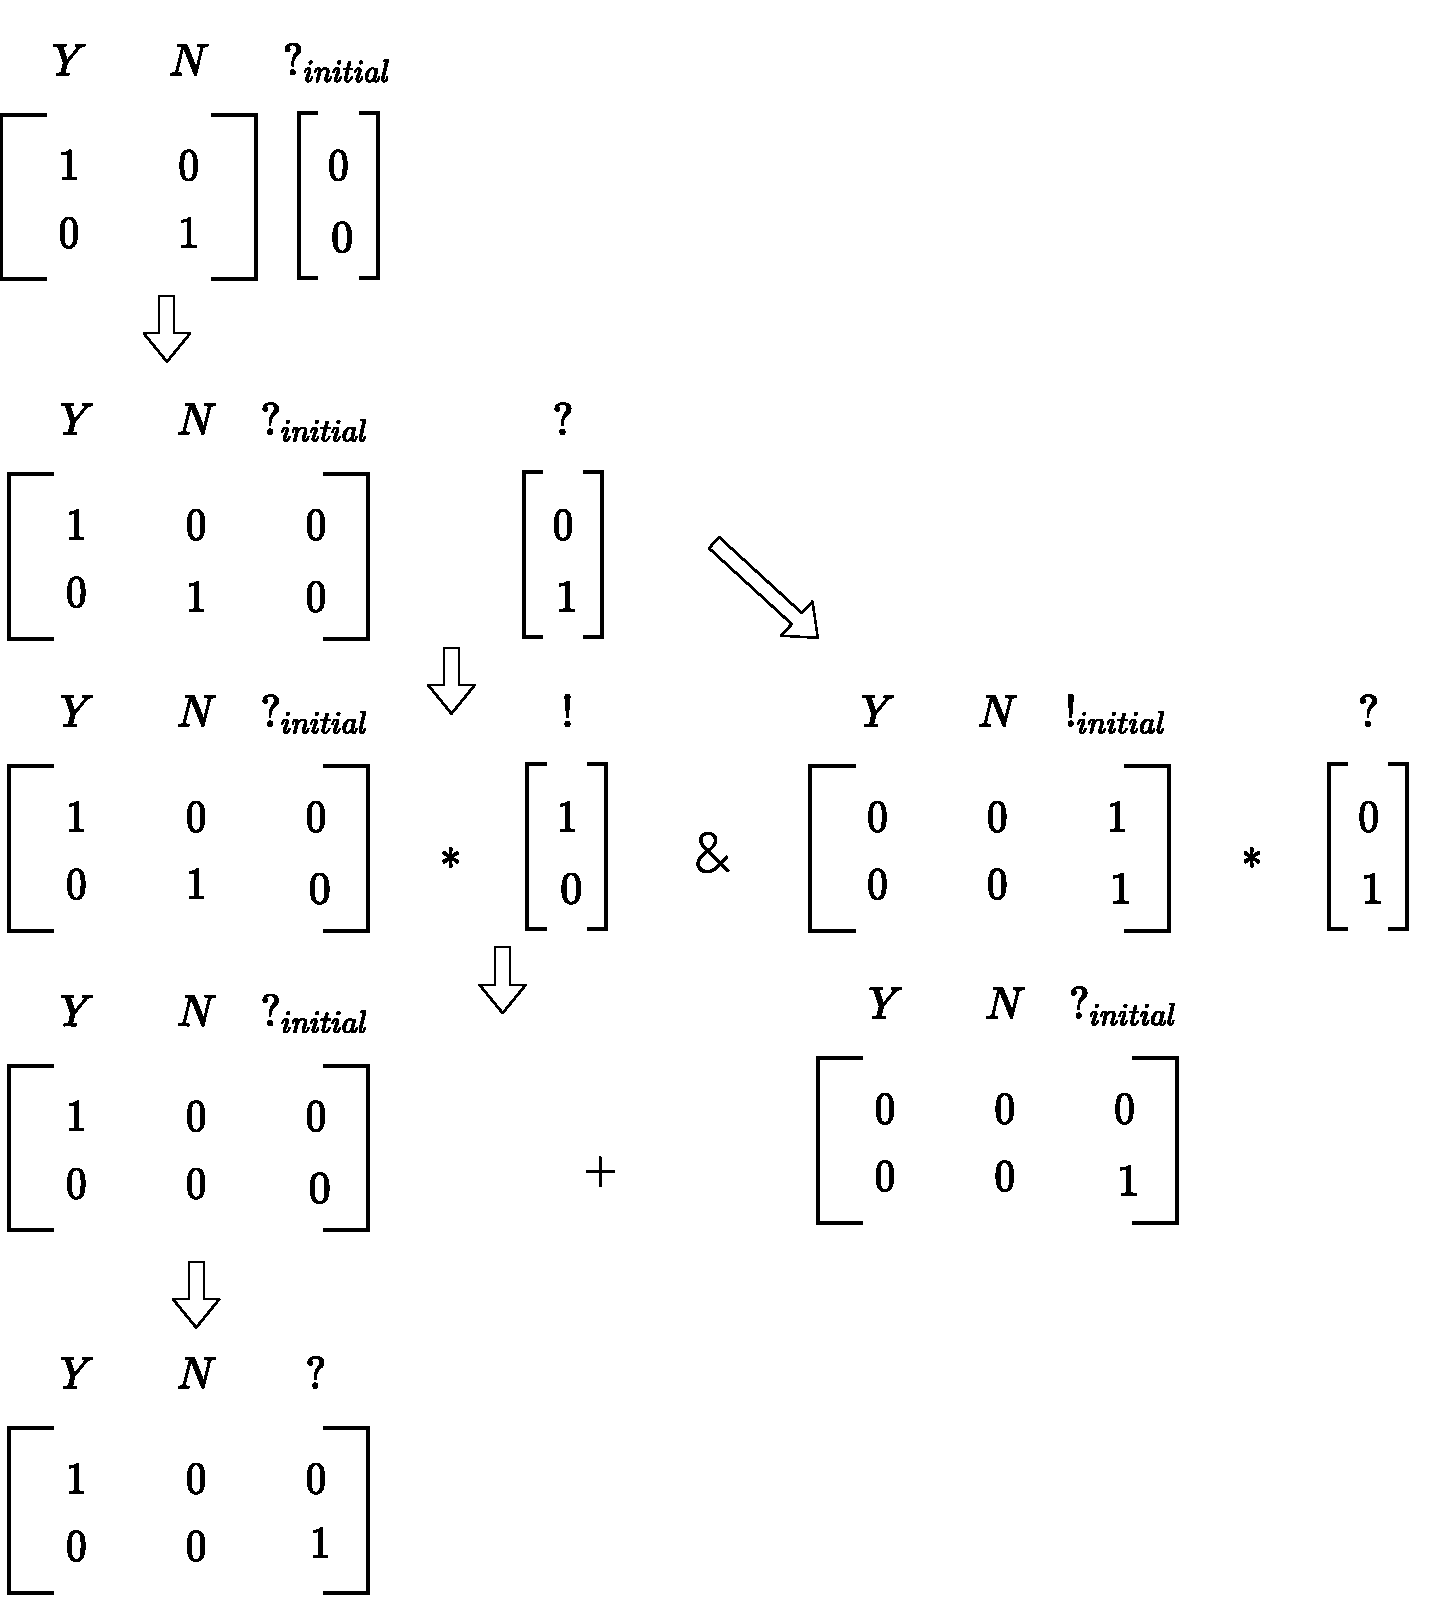
\includegraphics[width=1\textwidth]{images/extended_vocab.pdf} 
		\caption{The original answer by the AbL is merged with uncertainty information so that the answer for each attribute is either 'Yes', 'No' or '?'. Here we show a small example where attribute size is only $2$.}
		\label{fig:extended_vocab}
	\end{minipage}\hfill
	\begin{minipage}{0.45\textwidth}
		\centering
		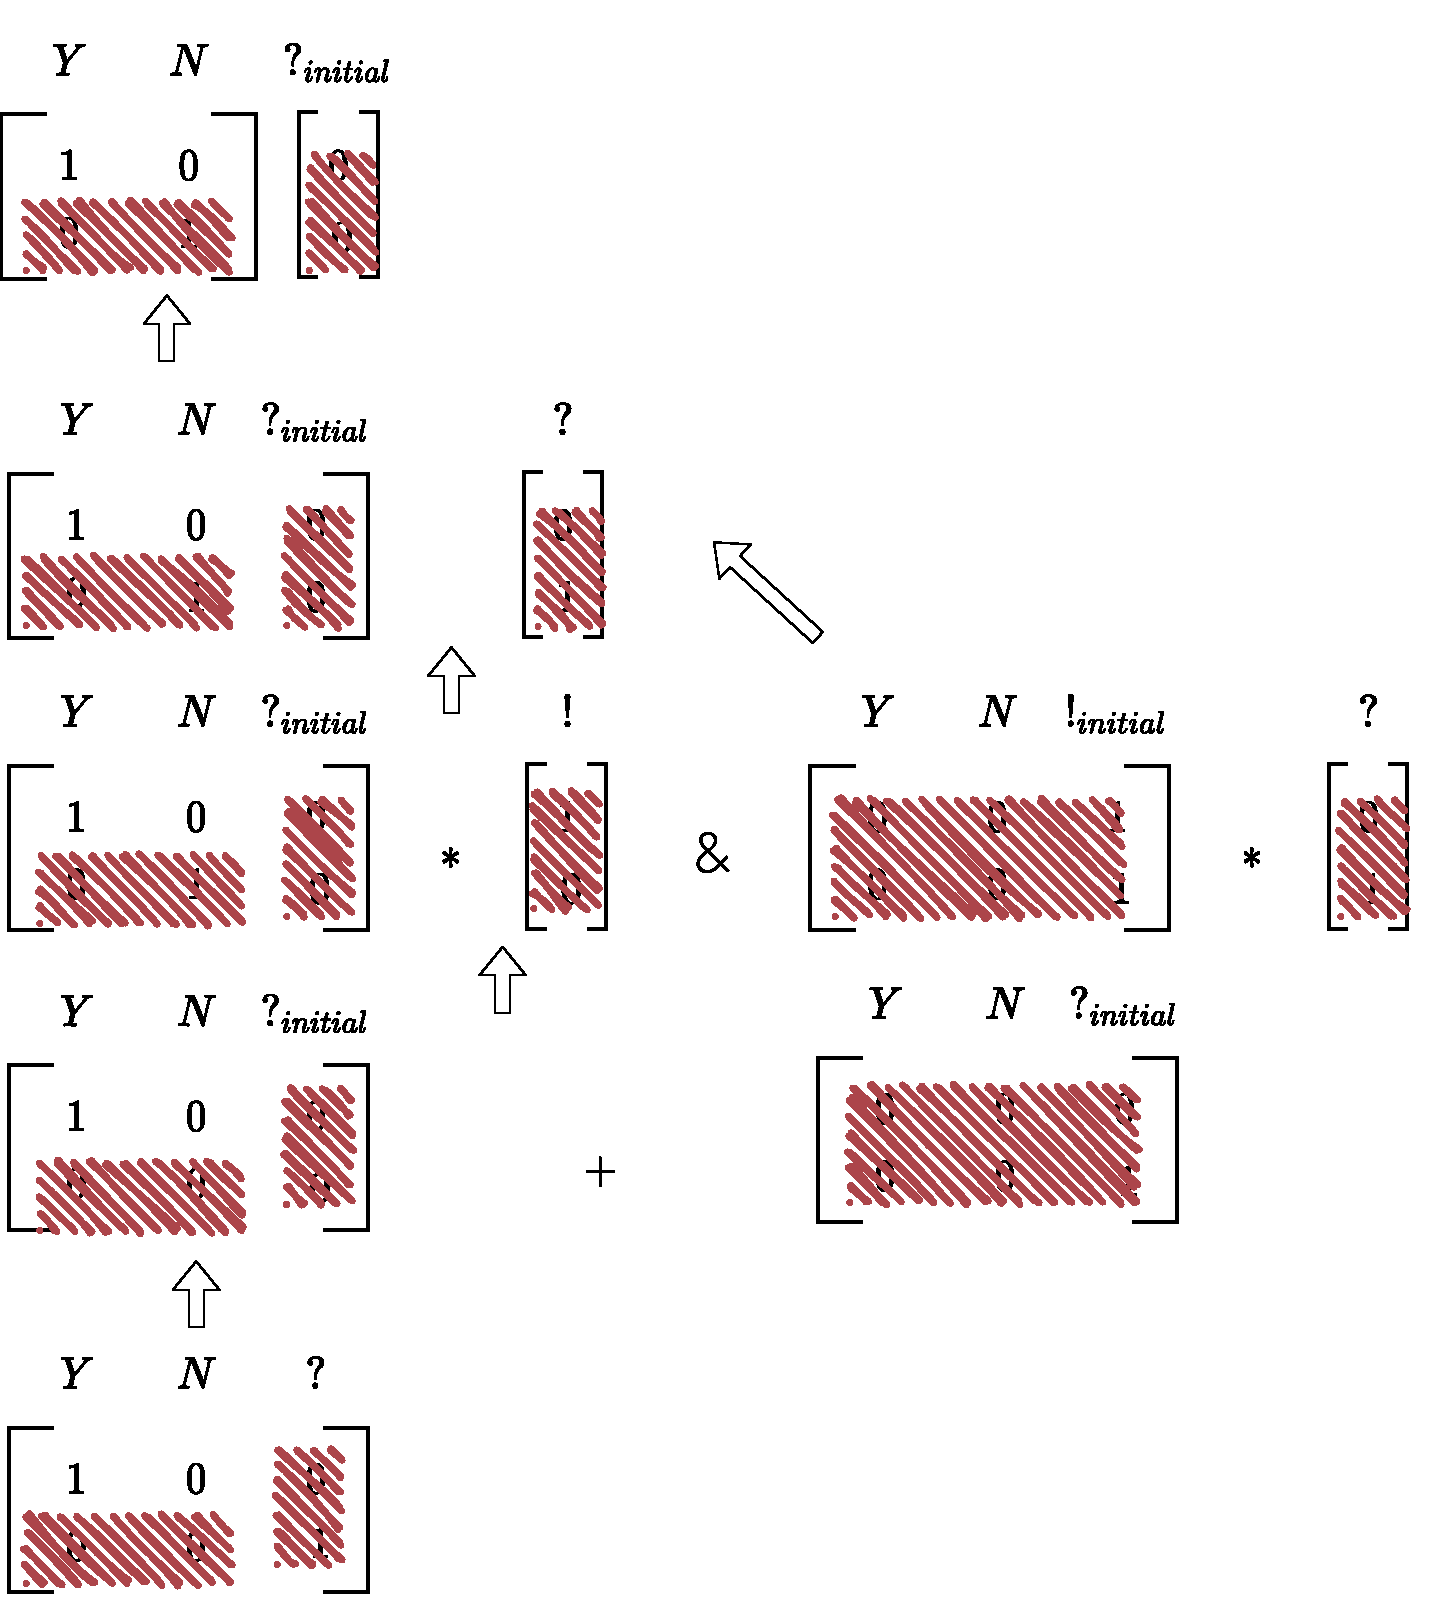
\includegraphics[width=1\textwidth]{images/extended_vocab_backward.pdf}
		\caption{Gradients coming from attributes that are deemed uncertain are detached from the computational graph. Other elements in the tensor are either $0$ (so are their respective gradients), or stem from leaf nodes.}
		\label{fig:extended_vocab_backward}
	\end{minipage}
\end{figure}
Here, we resort to an extended vocabulary of answers for $f_{AttrMLP}$. Instead of just 'Yes' and 'No', we also allow the AbL to answer with '?'. Thus $f_{AttrMLP}(z)$ should be $\in \lbrace 0,1 \rbrace^{num\_attributes \times 3}$. However, since, $f_{AttrMLP}(z) \in \lbrace 0,1 \rbrace^{num\_attributes \times 2}$ we need to append the uncertainty information to $d$ while avoiding conflicting answers. This process is shown, for a two attribute example in Figure \ref{fig:extended_vocab}. After receiving the output from $f_{AttrMLP} = d_{init}$ we initiate the uncertain column '?' with a vector of $0$'s and append this to the $d_{inint}$ to create $d_{temp}$. After computing uncertainty vector '?', we also create a negated version $!$ of it. This indicates all attributes where the model is certain. Subsequently, those are now used to clear rows. Vector '!' has $0$s where the model is uncertain. We use this to replace values in rows of uncertain attributes with $0$'s and get $d_{cleared}$. We also initiate a dummy tensor, that is of the same dimension as the $d_{cleared}$ and is all $0$s but in the column to the very right, where it is all $1$'s. Rows of this tensor are now cleared, using '?', wherever '?' has zeros, thus only rows with uncertain attributes remain and have a $1$ in the column responsible for uncertainty. Finally, this tensor and $d_{cleared}$ are added up to create our final decision $d$ which can now be indexed by the RDT.\\
When using this strategy in training, we need to make sure that no gradients come from uncertainty, so it is not misused and maximized in order for the model to profit from the additional column. We need to ensure that gradients only come from attributes, where the model is certain. For the operation, as described above, this is the case. We detach '?' and '!' from the computational graph. The dummy tensor is a leaf node, so no gradient is computed. Also, where values  in $d$ are $0$, their activation's derivative is $0$, so gradients are $0$. This is the case in rows of uncertain attributes. Which gradients are used and which are blocked in the previously used example is displayed in Figure \ref{fig:extended_vocab_backward}.




\subsection{Random Attribute Removal}
As a random baseline, to compare our remRDTC, and extRDTC to, we introduce 'random attribute removal' (randRDTC).
Similar to the remRDTC strategy, described in Subsection \ref{sec:remRDTC}, we prevent the RDT from asking questions. However, instead of blocking indices where uncertain attributes are, we randomly generate a tensor and block indices based on it. The probability of an index being blocked is similar to the probability of an attribute being deemed uncertain to allow fair comparison.




\chapter{Experiments}
\begin{figure}[t!]
	\centering
	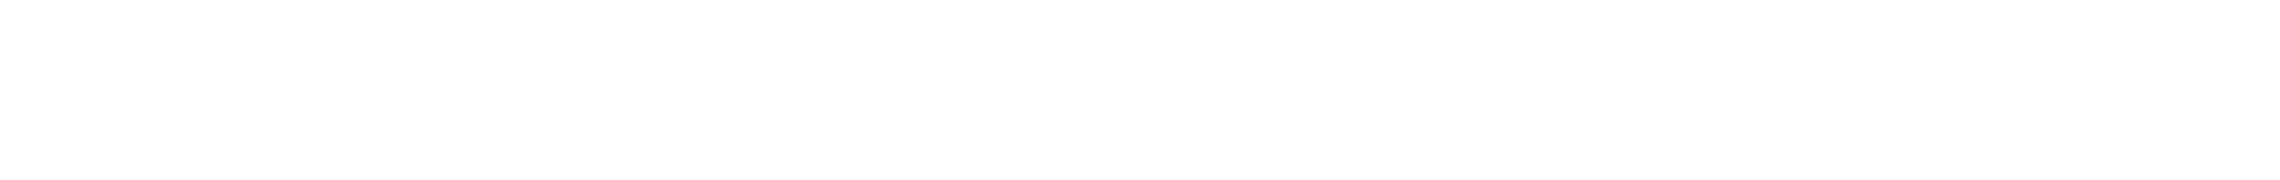
\includegraphics[width=1\textwidth]{images/attr_heatmap_short.pdf} 
	\caption{Normalized attributes misclassification frequency, uncertainty, and usage for attributes that are used by the model. Some of the attributes used frequently are highly uncertain. Attributes are denoted by their indices.}
	\label{fig:less_attrs}
\end{figure}
In this section, we briefly introduce the datasets used in our experiments. We present a quantitative evaluation of the model's uncertainty and its relation to other variables, such as attribute misclassification and attribute usage. Moreover, we investigate whether the model reliably yields high uncertainty for OOD examples. Finally, we evaluate our proposed model on benchmark image classification tasks. We compare the results to those of other explainable models and to current state of the art methods.


\section{Datasets}
We test our model on image datasets that provide attributes as side information. Popular datasets for this setting are Animals with Attributes 2 (AWA2) \cite{8413121}, aPY \cite{farhadi2009describing} and CUB \cite{WahCUB_200_2011}. Datasets with attributes are frequently used for zero- or few-shot learning tasks. In the explainable machine learning community, they are popular since attributes provide a human interpretable, natural language parameterization of image features.\\
% describe datasets in more detail
AWA2 is a medium scale coarse-grained dataset of 37,322 images that can be subdivided into 50 different classes of animals. Human annotators were tasked to label each image, choosing from 85 available attributes that describe each animal class. The aPY dataset is a small scale coarse-grained dataset that provides 15,339 images, annotated with 64 different attributes that describe each of the 32 classes. Finally, the most challenging dataset is the large scale fine-grained CUB. Here, the task is to classify 11,788 different images into 200 different classes. For this task, each image is annotated with 312 descriptive attributes.




\section{Investigating Uncertainties}
\begin{figure}
	\centering
	\begin{minipage}[t]{0.45\textwidth}
		\centering
		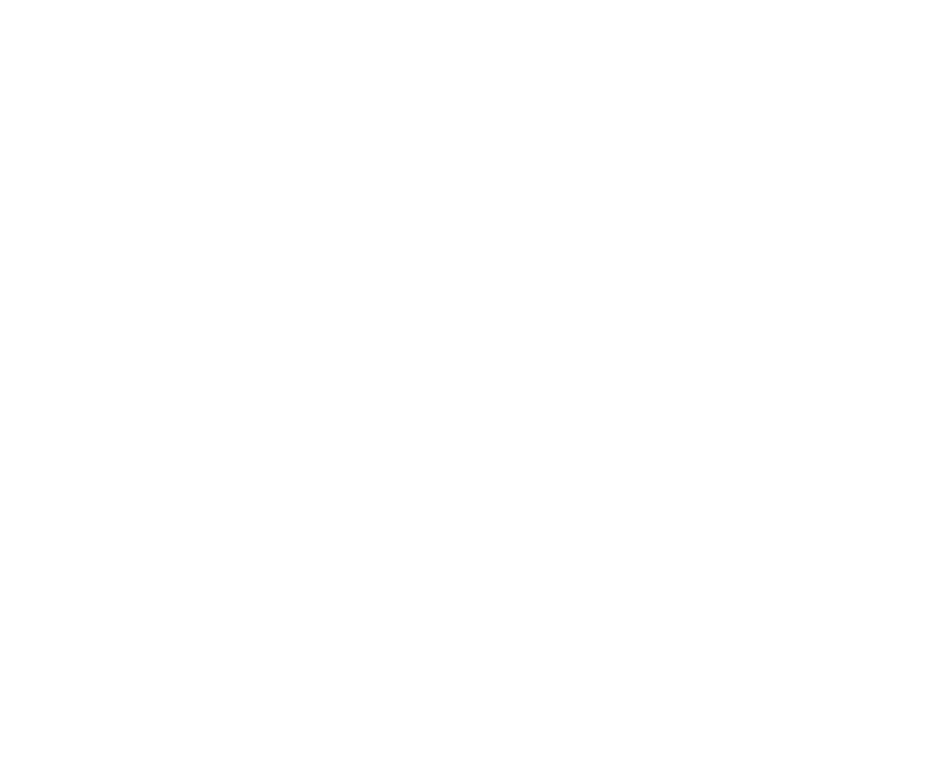
\includegraphics[width=1\textwidth]{images/corr_matrix.pdf}
		\caption{Correlations between misclassification rate, uncertainty, and usage of attributes.}
		\label{fig:corr_matrix}
	\end{minipage}\hfill
	\begin{minipage}[t]{0.45\textwidth}
		\centering
		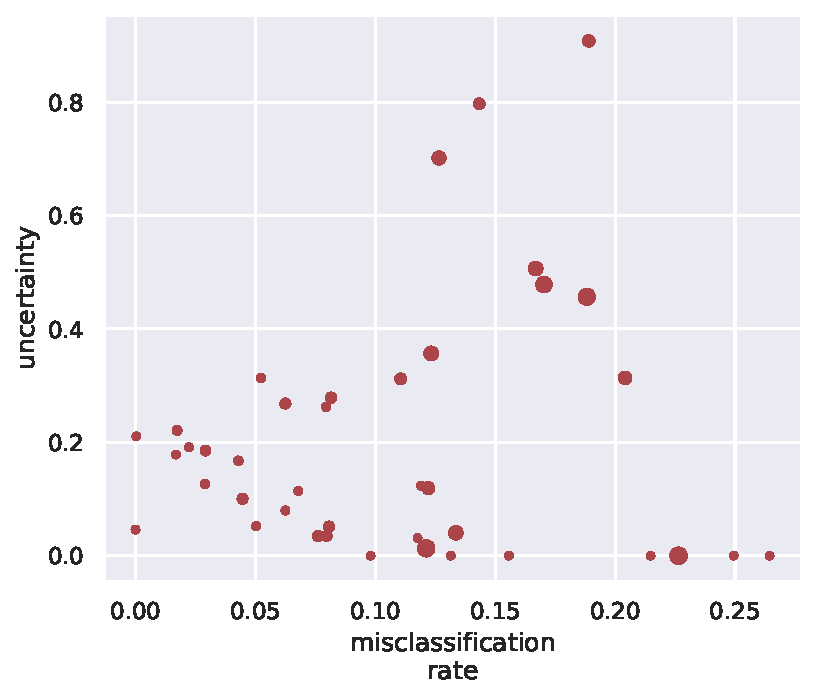
\includegraphics[width=1\textwidth]{images/error_sigma_corr_all.pdf} 
		\caption{Misclassification rates of attributes and their respective uncertainties. The size of the points represents how often they are used.}
		\label{fig:correlations}
	\end{minipage}
\end{figure}
%TODO have second look, once new figures are available
The purpose of the proposed model is not only to evaluate it on benchmark datasets but also to investigate uncertainties in the model. We examine correlations between variables such as attribute uncertainty, usage, and how often they are misclassified on the CUB dataset. From Figure~\ref{fig:less_attrs} it becomes obvious that only a small subset of the $312$ attributes is actually used to make decisions. We can already see, that most of the attributes that are used, however, are rarely misclassified. As apparent in the top row, all attributes here are quite reliably classified correctly. However, there seems to be no obvious correlation between uncertainty and misclassification as among the frequently used attributes (and thus reliably classified correctly) there are some attributes that have high uncertainty values.\\
In Figure \ref{fig:correlations} we can see that this is true and uncertain attributes appear among all levels of attribute accuracy. Figure~\ref{fig:corr_matrix} proves this  further as the correlation between the two is close to $0$. It also shows a negative correlation between attribute misclassification frequency and usage.
We can view misclassification frequency as inverse accuracy and thus have a positive correlation between usage and accuracy, suggesting that the model actively avoids attributes that it is likely to misclassify. Further, Figure~\ref{fig:corr_matrix} shows that there seems to be a positive correlation between usage and uncertainty. For one, this is due to attributes never used, having a low uncertainty, as the model is certain about them not being present. Futher, we hypothesize that the model uses highly discriminative attributes, even if it is uncertain about them.




\section{Testing on Out-of-domain Data}\label{sec:zero_shot}
An important aspect of our model is that it not only uses uncertainty information but that it can also express it. Detecting unknown data through high uncertainty could make such a model applicable for robust vision systems. In cases of high uncertainty a human could be consulted, thus preventing the model from making high-risk classifications without supervision. Here, we test whether examples, far from the training data cause high uncertainty.


\subsection{Attribute Zero Shot Setting}
%\begin{figure}[t!]
	%\centering
	%\begin{minipage}[t]{0.45\textwidth}
		%\centering
		%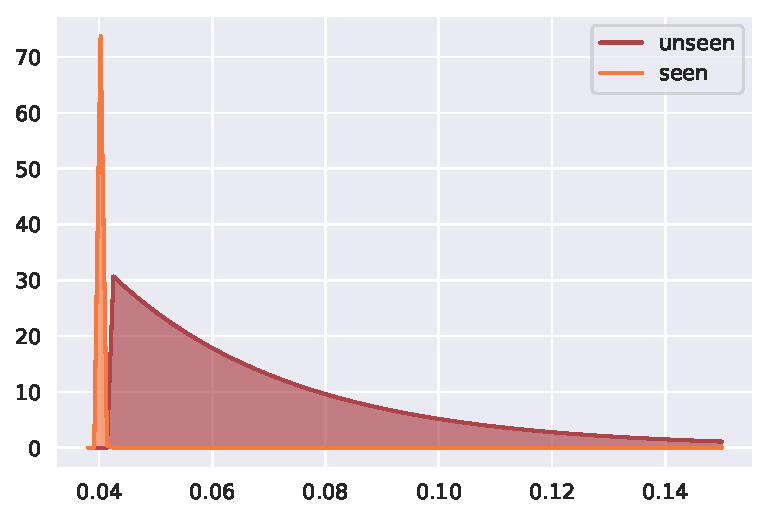
\includegraphics[width=1\textwidth]{images/attr_zero_shot_class_uncertainty.pdf} 
		%\caption{Maximum likelihood model for the exponential distribution of uncertainty %per example. Examples from classes that have unseen attributes have higher %attribute uncertainties.}
	%	\label{fig:unseen_attr_classes}
	%\end{minipage}\hfill
	%\begin{minipage}[t]{0.45\textwidth}
		%\centering
		%\includegraphics[width=1\textwidth]{images/zero_attr_class_uncertainty_hist_median%s.pdf}
		%\caption{Distribution of uncertainty values of seen and unseen attributes in %zero-shot-attribute setting (See Section \ref{sec:zero_shot}). The model is more %uncertain about attributes it has not encountered in the training set.}
%		\label{fig:unseen_attrs}
%	\end{minipage}
%\end{figure}
\begin{figure}[t!]
	\centering
		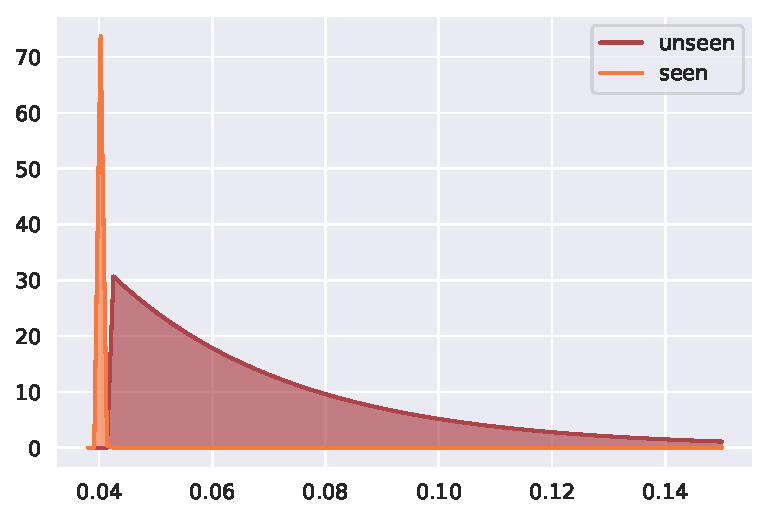
\includegraphics[width=0.7\textwidth]{images/attr_zero_shot_class_uncertainty.pdf} 
\caption{Maximum likelihood model for the exponential distribution of uncertainty per example. Examples from classes that possess unseen attributes have higher attribute uncertainties.}
\label{fig:unseen_attr_classes}
\end{figure}


As a sanity check, we first investigate attribute uncertainty in a zero-attribute setting. Therefore, we exclude certain classes from training data, so that some attributes are never seen by the model in training. For our setting, we use the CUB dataset, as it is the most challenging out of the introduced three. We construct a setting, where certain attributes do not occur in training data, and thus have to find classes, that have exclusive attributes. In CUB, we find a set of 24 classes that possess five exclusive attributes that do not occur in any of the other classes\footnote{This setting can be replicated by using the \textit{zero\_attr\_train\_test\_split.txt} file in the provided Github repository.}.\\
After training our model on the proposed split, we investigate uncertainties of classes that contain unseen attributes. We consider the mean uncertainty per example.
%For (2), we consider all uncertainty values of each attribute.\\
Figure \ref{fig:unseen_attr_classes} displays the modeled distribution of mean uncertainty per example, divided into classes that only posses attributes, occurring in the training data, and classes that possess 5 attributes, never encountered during training. We observe, that the latter have an overall higher uncertainty and a much wider variance, while the uncertainty values from seen attribute classes are concentrated.
%Displayed in Figure \ref{fig:unseen_attrs}, is the distribution of uncertainty values of attributes available during training, and the uncertainty values of attributes, unseen by the model, before the test stage. Here, we also observe an overall higher uncertainty for the latter.

\subsection{Zero Shot Setting}
Further, we investigate the uncertainty of our model in a classical zero-shot setting. We use a split of 150+50, where 150 classes are seen during training and validation. The remaining 50 classes are only seen in the test stage. We compare uncertainties for examples from classes seen during training to uncertainties of examples from unseen classes. Figure \ref{fig:zero_shot_uncert} shows that unseen classes generally have higher attribute uncertainty. This would allow the model to detect unseen classes with a high probability and notify a human user of its uncertainty.

%TODO check this 
%However, the overall most frequent uncertainty value is 0 for both classes. This is due to features, not present in the image, the corresponding attribute, typically the corresponding attribute(s) will yield low uncertainty.








\section{How does Our Model Compare?}\label{sec:results}
We compare our model to different other approaches, that either exemplify the current state of the art or are explainable.

\begin{figure}[t!]
	\centering
		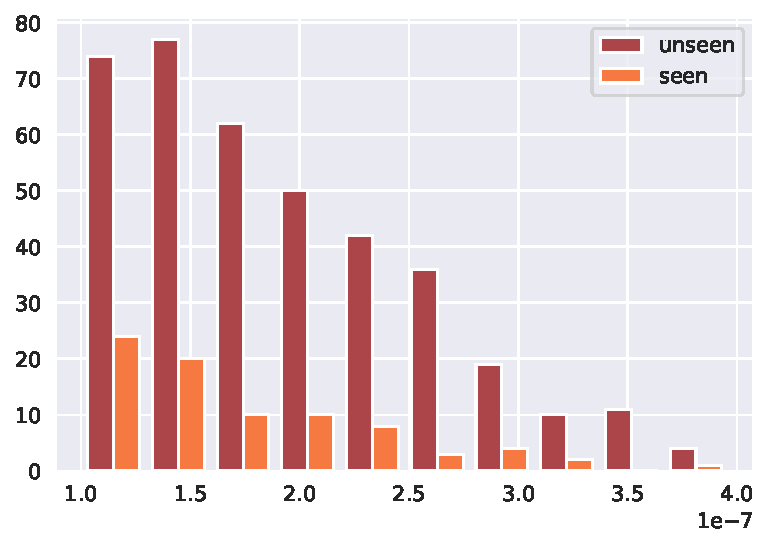
\includegraphics[width=0.7\textwidth]{images/zero_shot_class_uncertainty_median_hist.pdf}
\caption{Uncertainty values of attributes from seen and unseen classes. Examples from unseen classes have a higher attribute uncertainty. Attributes with an uncertainty value below $0.0000001$ are not shown.}
\label{fig:zero_shot_uncert}
\end{figure}



\subsection{Comparing RDTC to Other Models}
\begin{table*}[t]
	\renewcommand{\arraystretch}{1.3}
	\caption{We compare accuracy on AWA2, aPY, and CUB of our model and other methods. Standard deviations, denoted by $\pm$ are from five runs.}
	\label{tab:benchmarks}
	\begin{tabular*}{\textwidth}{c @{\extracolsep{\fill}} c c c c}
		%\hline
		&                                AWA2&          aPY&          CUB\\
		\hline
		\hline
		ResNet \cite{he2016deep}&       $98.2\pm 0.0$& $85.1\pm 0.6$ & $79.0\pm 0.2$ \\ 
		\hline 
		DT&                             $78.0\pm 0.4$&$64.3\pm 0.6$  & $19.3\pm 0.3$  \\ 
		\hline 
		dNDF\cite{kontschieder2015deep}&$97.6\pm 0.2$&$85.0\pm 0.6$ & $73.8\pm 0.3$ \\ 
		\hline 
		RDTC\cite{alaniz2019explainable}&$98.0\pm 0.1$&$85.7\pm 0.7$& $78.1\pm 0.2$   \\ 
		\hline 
		XDT&                            $73.9\pm 0.9$&$59.9\pm 1.5$  & $4.9\pm 1.3$ \\ 
		\hline 
		aRDTC\cite{alaniz2019explainable}&$98.6$&         $86.1$&  $77.9\pm 0.6$\\ 
		\hline
		remRDTC(ours)&          $98.7$          &          $86.4$&  $77.7$\\ 
		\hline
		extRDTC(ours)&          $98.7$          &          $85.4$&  $77.8$\\
		%\hline 
	\end{tabular*}
\end{table*}
ResNet-152 \cite{he2016deep} is not explainable. Here, the ResNet was pre-trained on ImageNet data \cite{deng2009imagenet} and then fine-tuned for the specific tasks. We also use a ResNet trained in this manner in our proposed model to extract features from images. When we train the remRDTC and extRDTC models, we keep the weights in the ResNet fixed and only adjust all other parameters in the model.\\
XDT and DT are both traditional decision tree models that serve as a baseline. For DT \citet{alaniz2019explainable} propose the following method: DT is given features extracted by the previously introduced pre-trained ResNet. Splits are created according to values in the extracted feature vector. For each split, one feature is chosen and a split is created. This is repeated until either each leaf node corresponds to exactly one class or an early stopping-criterion is met. \\
Moreover, \citet{alaniz2019explainable} introduce XDT, where each split is given a semantic meaning, for the splits to correspond to interpretable attributes and not only features. The XDT is therefore not given features, directly stemming from the ResNet, but attributes, learned by an MLP that was trained to predict attributes from ResNet features (similar to $f_{AttrMLP}$). They train both DT and XDT using the CART algorithm \cite{breiman1984classification}. As a splitting criterion, they chose the Gini impurity index over entropy-based methods due to its computational advantage \cite{raileanu2004theoretical}.
Another explainable model is Deep Neural Decision Forest (dNDF), proposed by \citet{kontschieder2015deep}. They learn an ensemble of trees by optimizing routing probabilities in each tree's internal nodes. Every path through a tree eventually leads to class distribution, represented in leaf nodes. All internal nodes are sigmoid-activated, differentiable stochastic functions, parameterized by an optimizable $\theta$. The final prediction is an average over the resulting decision tree forest. One downside of the resulting averaged stochastic routing decisions is the reduced interpretability as they allow for multiple possible routes. The RDTC models only yield one possible route for a given example. Therefore, we consider only an dNDF using a single tree instead of an ensemble mean.\\
The results are stated in Table~\ref{tab:benchmarks}. We see that both strategies of our model outperform other explainable methods. The achieved accuracy is similar to that of the original RDTC model and is comparable to that of unexplainable state-of-the-art methods such as ResNet. 




\subsection{Comparing Different RDTC Models}
We evaluate different configurations of our model on the three datasets. We compare the original RDTC model to models using our two proposed strategies of remRDTC and extRDTC. We also include randRDTC as a baseline that randomly removes attributes, based on the average probability of an attribute having an uncertainty higher than the specified threshold. Additionally to class accuracy, we also consider the model's attribute accuracy. For all versions, we use $\lambda=0.2$. The results are displayed in Table~\ref{tab:iterations}. We can see, that aRDTC, remRDTC, and extRDTC achieve similar class accuracies while the randRDTC strategy has a slightly lower class accuracy in most experiments. Our model has higher attribute accuracies (except for extRDTC on AWA2). %We hypothesize that this is due to the model avoiding using high-risk attributes. 
%TODO think about last sentence again when new correlation matrix is available




\begin{table*}[t]
	\caption{Class and attribute accuracy on three benchmark datasets. We compare the original aRDTC model to three different strategies of our proposed model.}
	\label{tab:iterations}
	\begin{tabular*}{\textwidth}{c  @{\extracolsep{\fill}}c c c c}
		& aRDTC \cite{alaniz2019explainable} & Random Baseline & remRDTC & extRDTC \\ 
		%\hline 
		%\hline
		\textbf{AWA2}& & & &\\\hline\hline
		Class &  98.6&  98.5&  98.7&  98.7\\ 
		\hline 
		Attribute & 80.4 & 84.6 &  87.5&  82.31\\ 
		&  &  &  &  \\
		\textbf{aPY}& & & &\\\hline\hline
		Class & 86.1&  86.5&  86.4&  85.4\\ 
		\hline 
		Attribute &  86.4&  86.2&  87.6& 87.12 \\ 
		&  &  &  &  \\ 
		\textbf{CUB}& & & &\\\hline\hline
		Class &  77.9& 76.8 & 77.7 & 77.8 \\ 
		\hline 
		Attribute &  68.6&  70.0& 77.4 & 82.6 \\ 
		&  &  &  &  \\ 
	\end{tabular*}
\end{table*}







\chapter{Discussion}
Uncertainty estimation in deep learning is not trivial. It is an active topic of research and therefore subject of ongoing change and discussion. We will critically reflect on our work and discuss whether epistemic uncertainty (that is only considering attributes) is useful in our setting and how we could alleviate remaining issues. We also take a look at a hypothetical example, on how uncertainty information could be used.


%\section{Increased Convergence Time}
%Both of our proposed models have longer convergence time as the original RDTC, proposed by \citet{alaniz2019explainable}. We hypothesize why this might be the case for our model.\\
%In both strategies we prevent the model from using gradients, coming from uncertain attributes. The model thus has less gradient information available. As a direct result, the model can update fewer parameters in each step, or make smaller changes. We hypothesize that this causes increased convergence time. 



\section{The Right Kind of Uncertainty?}
In our approach, we only consider epistemic uncertainty, which is the uncertainty arising from variance in the model's parameters. However, in closed datasets, as the ones considered, epistemic uncertainty will not change very much after the model has seen every training example. Not considering data augmentation techniques, this happens within one epoch. %TODO hmmm


\subsection{Estimating Heteroscedastic Uncertainty}
Heteroscedastic is a function of data and thus can be learned. \citet{kendall2017uncertainties} propose to learn an additional output $\sigma^2$ and a loss function:
\begin{align}
\mathcal{L}(\theta) = \frac{1}{N}\sum_{i=1}^{N} \frac{||y_i-f(x_i)||^2}{2\sigma(x_i)^2} + \frac{1}{2}log\;\sigma(x_i)^2.
\end{align}
If a prediction is wrong, it encourages a high value for $\sigma^2$, thus lowering its impact. In a variational inference setting (which our dropout model is corresponding to) for classification with sample size $T$, \citet{kendall2017uncertainties} propose to model aleatoric uncertainty as:
\begin{align}
&\frac{1}{T}\sum_{t=1}^{T}diag(\hat{\sigma}_t^2).
\end{align}
Alternatively, a different approach was proposed by \citet{kwon2020uncertainty} that does not require learning $\sigma^2$. 
\begin{align}
\label{eq:approx}
&\frac{1}{T}\sum_{t=1}^{T}diag(\hat{p}_t) - \hat{p}_t\hat{p}_t^T,
\end{align}
where $\hat{p}_t = softmax(\pi)$  and $\pi$ are the unscaled logits.
This is an approximation to the variational posterior:
\begin{align}
\label{eq:variational_predictive}
\int_{\Omega}\left[ diag (\mathbb{E}_{p(y^*|x^*,w)}[y^*]) -\mathbb{E}_{p(y^*|x^*,w)}[y^*] \cdot \mathbb{E}_{p(y^*|x^*,w)}[y^*] \right]q_{\theta}(w)dw,
\end{align}
which is the diagonal of the expected outputs, subtracted by the product of the expected outputs with themselves, and finally multiplied with the variational posterior over the weights $w\in \Omega$.  For $T\rightarrow \infty$, equation \ref{eq:approx} will converge to equation \ref{eq:variational_predictive}.


\subsection{Risk versus Uncertainty}
\citet{osband2016risk} suggests to distinct the variance arising from dropout neural networks, from actual uncertainty. He  criticizes that the posterior, approximated through the mean and the variance form multiple forward passes does not concentrate as more data becomes available. According to him, this variance is rather associated with what is called risk in decision theory. There, the term risk refers to the inherent stochasticity of a model. However, this is what we previously introduced as epistemic uncertainty. This issue is thus rather about semanticity. We, therefore, acknowledge it but stick to the convention of differentiating between epistemic and aleatoric uncertainty.


\subsection{Beyond Attribute Uncertainty}\label{sec:attr_uncertainty}
As the only point, where uncertainty information is retrieved in our model is in the $f_{AttrMLP}$ which maps ResNet features to attributes, our model can only consider attribute uncertainty. Thus, as soon as an attribute is encountered in training, its uncertainty should converge. This may be unhelpful in realistic scenarios, where an unknown class is encountered that can be described by a set of known attributes as such an example would not yield high uncertainty. Replacing $f_{ClassMLP}$ with a Dropout MLP and computing uncertainty there as well may potentially alleviate this issue and could allow further insights.\\
Note that this is considering that outputs learned by the $f_{AttrMLP}$ would directly correspond to attributes. This is likely not the case. As for one, we use attribute coefficient $\lambda=0.2$ in all our settings, and second, learning such a direct mapping between feature and attribute space is not a trivial problem. %TODO citation needed


\begin{figure}[t]
	\centering
	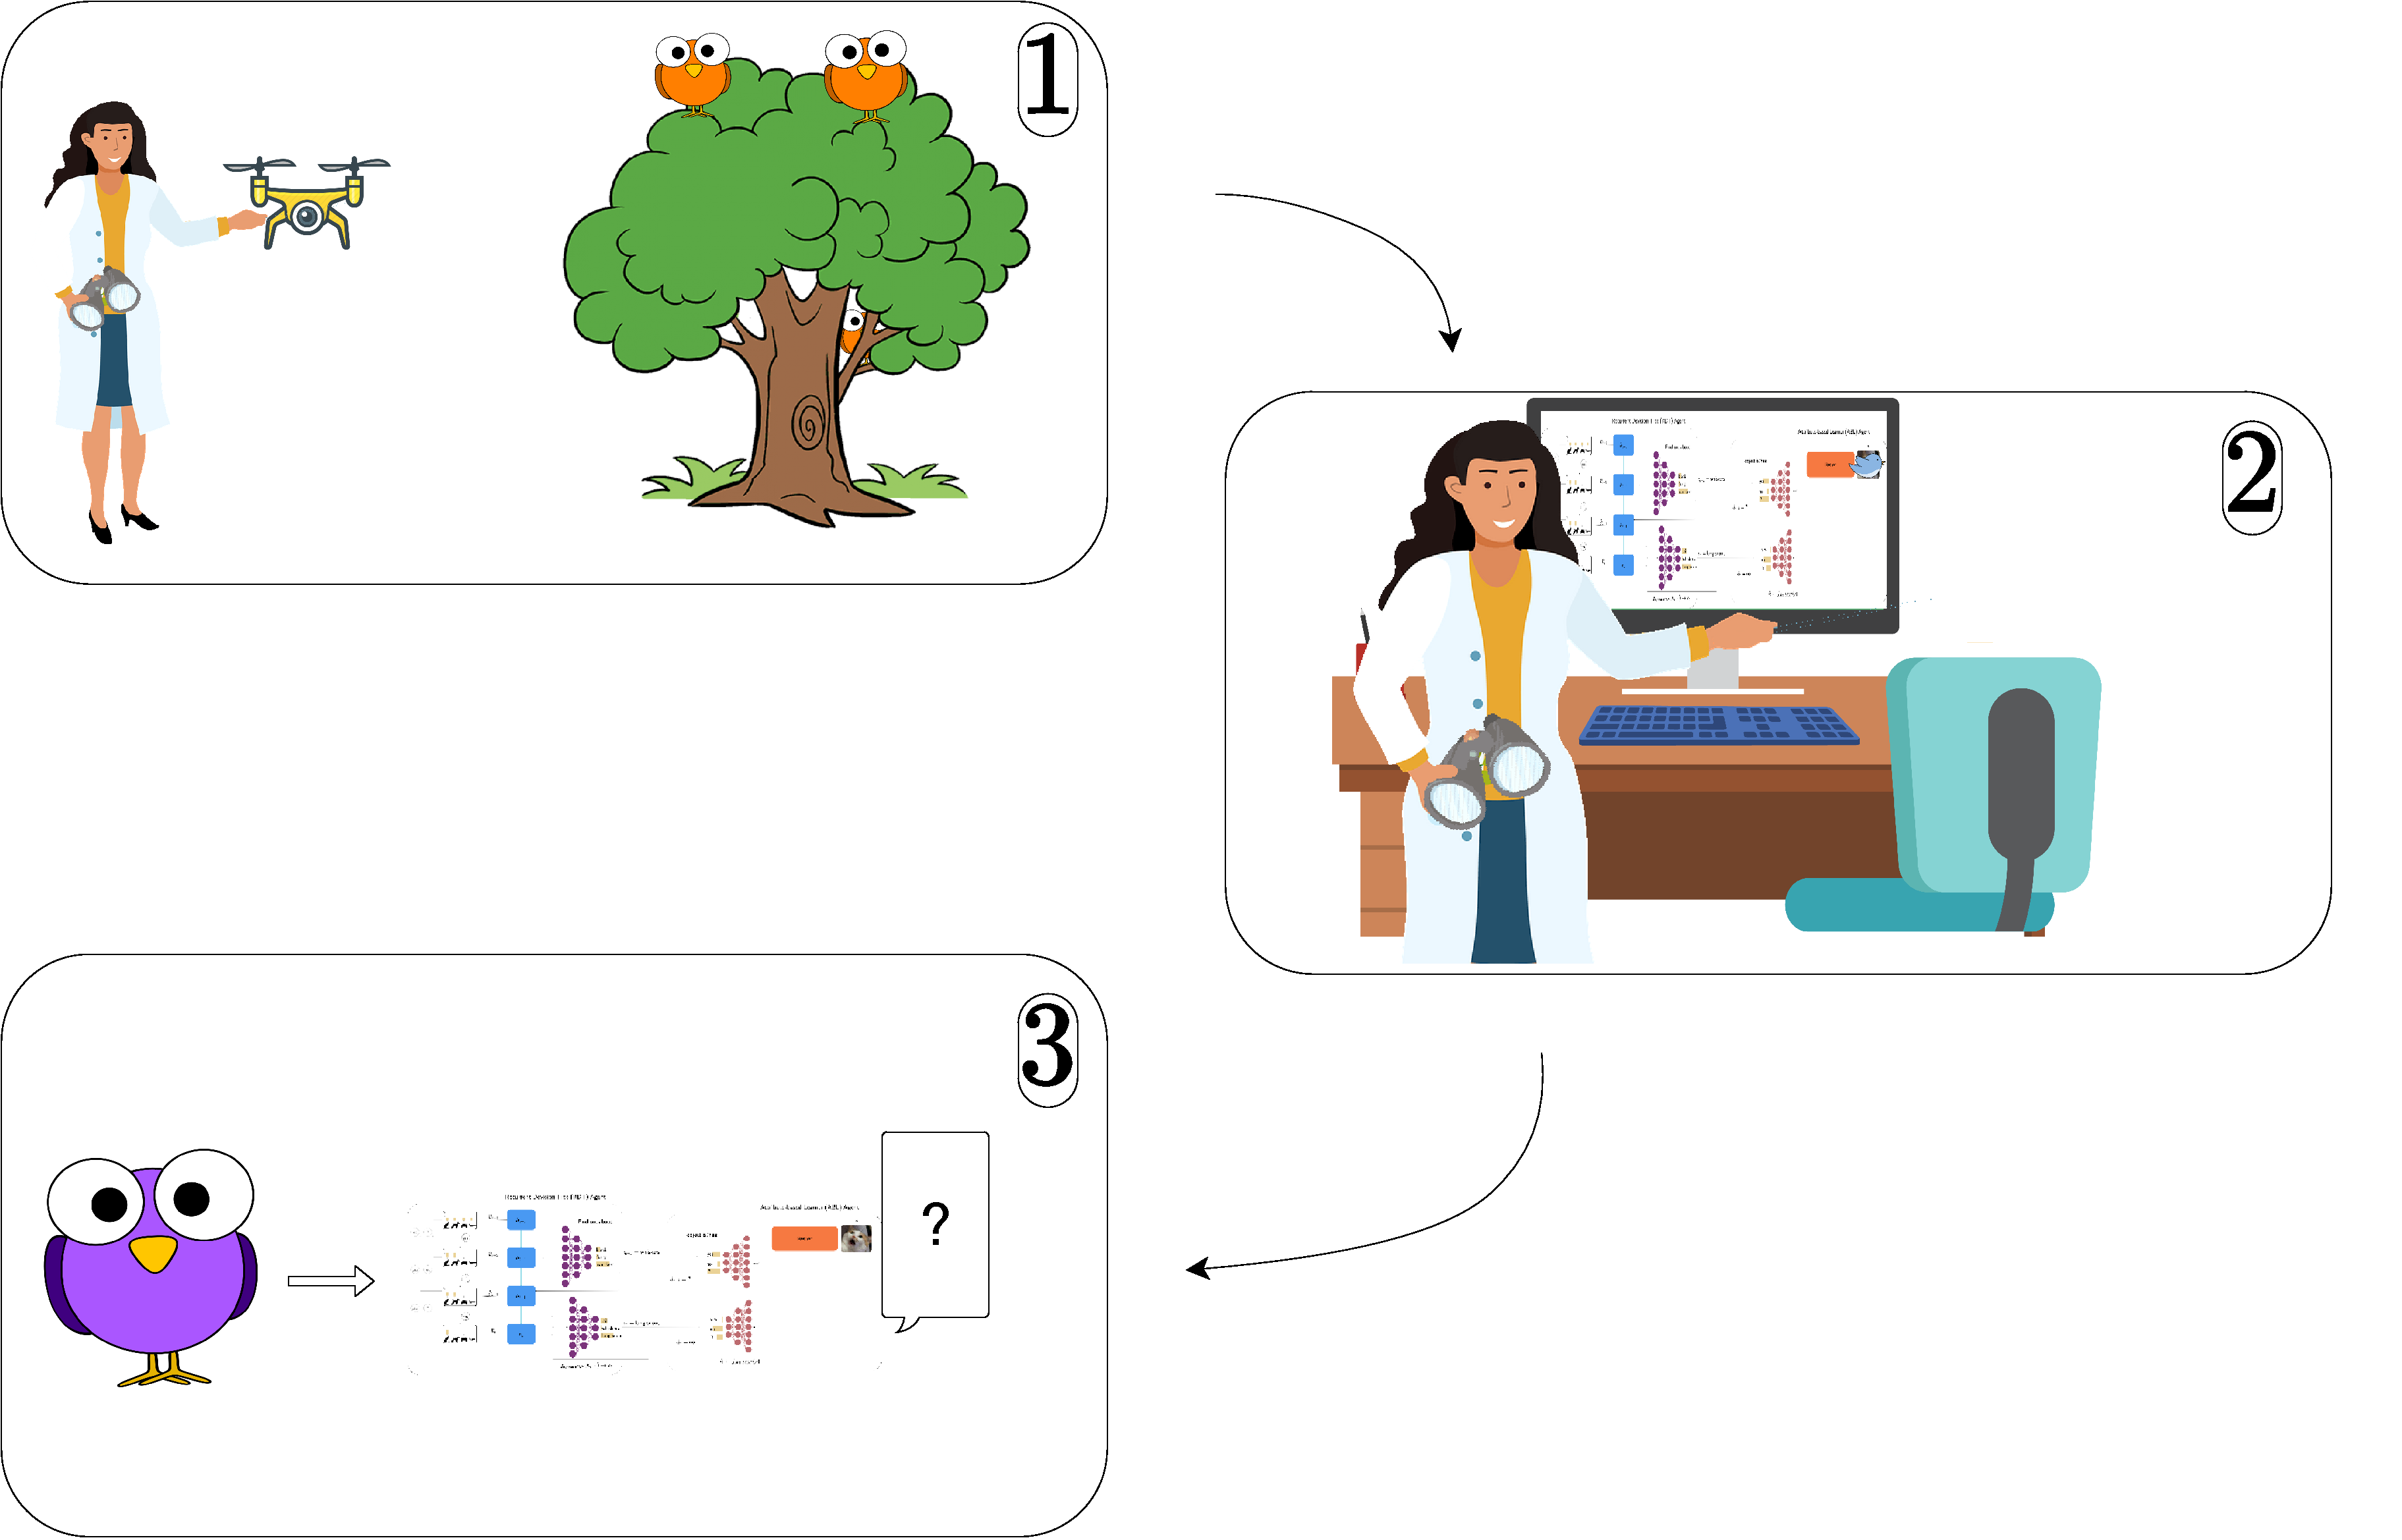
\includegraphics[width=0.9\textwidth]{ornithology.pdf}
	\caption[caption for ]{After collecting images of birds, the ornithologist lets our proposed model classify the vast amount of data. Only in cases of high uncertainty, she is consulted and can classify the image manually. \footnotemark}
	\label{fig:qual}
\end{figure}
\footnotetext{Graphics derived from \cite{cartoon2016desk, teacher2016, binocular2016, drone2016,bird2016}.}

\section{A Practical Example}
In the previous sections, we introduced a model that reliably can express its uncertainties to a user in an explainable decision process. In a realistic setting, this could provide the user with valuable insights. Instead of only yielding the final classification and an explanation tree, the model can also tell the user how uncertain it is about each part of the tree. If the user sees that the model was uncertain about several attributes it used, the classification may be done manually.\\
Let's consider an example (displayed in Figure \ref{fig:qual}) where an ornithologist is tasked to do a comprehensive survey of bird species and their respective numbers. Since our ornithologist is not given any helper, she decides to use a drone and a computer vision software that takes a picture of every bird it encounters (1). After letting the drone fly around in the survey area for some days, the ornithologist inspects the data and finds that the drone collected so much data that it hardly can be examined manually. Luckily, she has heard of our model and decides to use it on the data(2). For each image, the model yields a classification and an explanation. However, due to climate change, some bird species that typically do not occur in the survey area have made their way into the collected data. The model has never seen such birds as they typically only appear much further south. It is highly uncertain and notifies the ornithologist (3). The ornithologist sees that this species is unknown to the model and thus rendered it uncertain, unable to make a reliable classification. However, since she knows of this species she can quickly classify it manually.

% ornithology example 


\section{Carbon Footprint Estimation}
% devices
To produce our results, we relied on GPU's provided by the University of Tübingen ML Cluster of Excellence and Google. We are aware of the profound impact of emissions caused, on the world's climate.
The GPU's provided by Google were Nvidia Tesla K80 which operate up to the thermal design power of $300\;W$ \cite{nvidia2015tesla}. Devices of the University of Tübingen GPU cluster are Tesla V100-SXM2 which, at full capacity, operate up to a thermal design power of $300\;W$ \cite{nvidia2017tesla}. These specifications are without considering cooling and additional computational units. We assume these additional devices to operate at $50\;W$.\\
% epochs
While no single model was trained for more than $100$ epochs on any dataset, if we consider all models and all iterations of models, we have amassed circa $5000$ epochs of training. Mean training time for one epoch was approximately $6$ minutes, or in $1$ hour, a model could be trained for $10$ epochs. Thus for $5000$ epochs, we amass $500$ hours of training time. Considering the specification of our GPUs and assuming they are running at full capacity, we get an upper bound of $500\;h * (300\;W + 50\;W) = 175000\;Wh=175\;kWh$ of energy consumption.\\
% co equivalent
The German federal office for environmental concerns (Umweltbundesamt) estimates the amount of $CO_2$ necessary to produce one kilowatt-hour to be $401\;g$ \cite{icha2016entwicklung}. Considering, we required $175\;kWh$, this would result in the $CO_2$ equivalent of $401\;g \cdot 175 = 70175\;g \approx 70\;Kg$.

%TODO check watt or kilowatt

\begin{figure}[t]
	\centering
	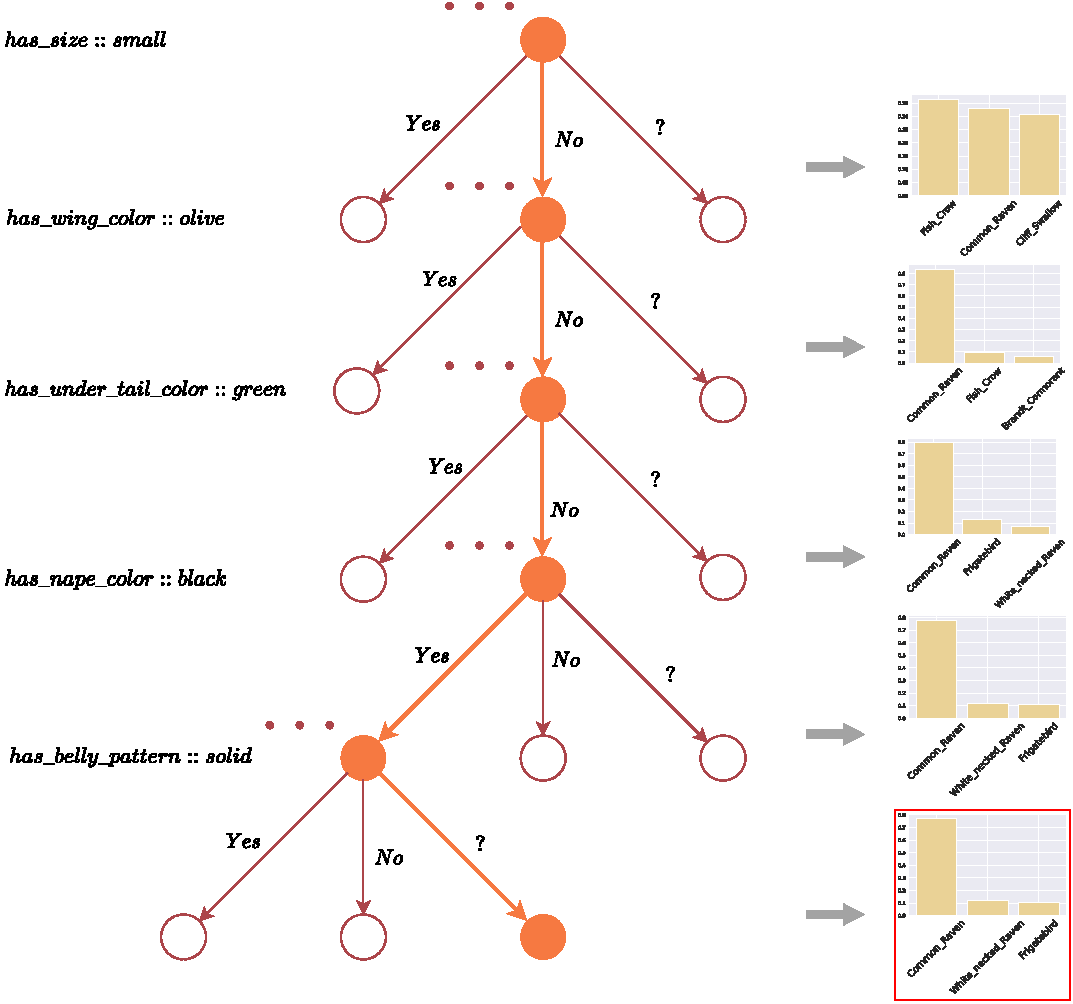
\includegraphics[width=1\textwidth]{images/example_tree.pdf}
	\caption{Five steps of a extRDTC decision process. The model has used an uncertain attribute and the final classification is wrong. In such a case, a human user could be consulted and manually classify the image. Note that the the softmax classification output is highly confident despite being wrong.}
	\label{fig:example_tree}
\end{figure}

\chapter{Conclusion}
Extending the work of \citet{alaniz2019explainable}, we propose an explainable model that is aware of and can express its uncertainties. The original model delivers a binary decision tree as an explanation, leveraging human-interpretable attributes provided as side information. The nodes of the resulting tree correspond to attributes and the edges to either 'Yes' or 'No' answers regarding the presence of these attributes. In our work, we give the model the ability to either avoid uncertain attributes to be used in the decision tree or extend it to a ternary decision tree, where '?' is an additional option.\\
While our proposed extension does not outperform the original RDTC model, our remRDTC and extRDTC still outperform other explainable methods such as decision trees or dNDF. Moreover, the performance is comparable to that of unexplainable state of the art methods, such as ResNet.\\
Our model does not only utilize uncertainty information but also allows introspection. We use this to further investigate the relationship between attribute usage, misclassification, and uncertainty.
We show that our model reliably yields high uncertainty for unseen attributes and classes. This would allow the model to consult a human user in cases of high uncertainty, thus making it more applicable in real-world scenarios than comparable methods.
Finally, we critically reflect on the weaknesses of the model and propose possible improvements for future work.



\bibliographystyle{alpha}
\bibliography{bibliography}




\chapter*{Acknowledgments}
I would like to thank my pet snake, which sleeps all day, and my mother, who is the hardest working person I know. I would like to thank Zeynep and Stephan for the continuous support, critical questions, and helpful insights.



\chapter*{Selbstst\"andigkeitserkl\"arung}
Hiermit versichere ich, dass ich die vorliegende Bachelorarbeit selbst\"andig und
nur mit den angegebenen Hilfsmitteln angefertigt habe und dass alle Stellen,
die dem Wortlaut oder dem Sinne nach anderen Werken entnommen sind,
durch Angaben von Quellen als Entlehnung kenntlich gemacht worden sind.
Diese Bachelorarbeit wurde in gleicher oder \"ahnlicher Form in keinem anderen
Studiengang als Pr\"ufungsleistung vorgelegt.

\vspace*{8ex}
\hrule
\vspace*{2ex}
Stefan Wezel (Matrikelnummer 4080589), \today

\end{document}

